% When submitting your files, remember to upload this *tex file, the pdf generated with it, the *bib file (if bibliography is not within the *tex) and all the figures.

% NB logo1.jpg is required in the path in order to correctly compile front page header %%%

\documentclass[utf8]{FrontiersinHarvard} % for articles in journals using the Harvard Referencing Style (Author-Date), for Frontiers Reference Styles by Journal—https://zendesk.frontiersin.org/hc/en-us/articles/360017860337-Frontiers-Reference-Styles-by-Journal
\usepackage{url,hyperref,lineno,microtype,subcaption}
%\usepackage[]{natbib, booktabs, graphicx, tabularx, makecell}
\usepackage{booktabs}
\usepackage{lscape, float, multirow, adjustbox}
\usepackage[T1]{fontenc}
\usepackage[onehalfspacing]{setspace}
\usepackage{graphicx} 

\linenumbers


% Leave a blank line between paragraphs instead of using \\


\def\keyFont{\fontsize{8}{11}\helveticabold }
\def\firstAuthorLast{Morris {et~al.}} %use et al only if is more than 1 author
\def\Authors{Joanna Morris\,$^{1,2,*}$, Emma Kealey\,$^{2,3}$, Frankie Greene\,$^{1,4}$, Joemari Pulido\,$^{2,5}$, Tess Rooney\,$^{2,6}$, Ethan Moore\, $^{2}$, Crismar Ramos-Marte\, $^{2}$, Natalia Alzate\,$^{2}$}
% Affiliations should be keyed to the author's name with superscript numbers and be listed as follows—Laboratory, Institute, Department, Organization, City, State abbreviation (USA, Canada, Australia), and Country (without detailed address information such as city zip codes or street names).
% If one of the authors has a change of address, list the new address below the correspondence details using a superscript symbol and use the same symbol to indicate the author in the author list.
\def\Address{$^{1}$School of Cognitive Science, Hampshire College, Amherst, MA, USA \\
	$^{2}$Department of Psychology, Providence College, Providence, RI, USA \\
	$^{3}$Department of Linguistics, University of Southern California, Los Angeles, CA, USA \\
	$^{4}$Oregon Health \& Science University and Portland State University School of Public Health, Portland, OR, USA \\
	$^{5}$Department of Cognitive, Linguistic \& Psychological Sciences, Brown University, Providence, RI, USA \\
	$^{6}$Columbia University School of Nursing, New York, NY, USA}
% The Corresponding Author should be marked with an asterisk
% Provide the exact contact address (this time including street name and city zip code) and email of the corresponding author
\def\corrAuthor{Joanna Morris}

\def\corrEmail{jmorris6@providence.edu}


\begin{document}
	\onecolumn
	\firstpage{1}
	
	\title[Running Title]{Reading skill and the time course of morphological processing: electrophysiological evidence for stage-specific modulation} 
	
	\author[\firstAuthorLast ]{\Authors} %This field will be automatically populated
	\address{} %This field will be automatically populated
	\correspondance{} %This field will be automatically populated
	
	\extraAuth{}% If there are more than 1 corresponding author, comment this line and uncomment the next one.
	%\extraAuth{corresponding Author2 \\ Laboratory X2, Institute X2, Department X2, Organization X2, Street X2, City X2 , State XX2 (only USA, Canada and Australia), Zip Code2, X2 Country X2, email2@uni2.edu}
	
	
	\maketitle
	
	
	
	
\begin{abstract}
		
		%%% Leave the Abstract empty if your article does not require one, please see the Summary Table for full details.
	\section{}
	Skilled reading of morphologically complex words depends on both high-quality lexical representations and sensitivity to morphological structure. However, we do not yet understand how these abilities shape the time course of morphological processing. In this study, event-related potentials (ERPs) and reaction times were recorded during a lexical decision task on morphologically complex words and nonwords; both varied in base frequency and family size, and nonwords additionally varied in morphological complexity. Individual differences were quantified via principal components analysis of vocabulary knowledge, spelling ability, and print exposure, yielding two orthogonal dimensions: Language Proficiency and Orthographic Sensitivity. Behaviourally, response times were sensitive to base frequency and family size for words, and to morphological complexity for nonwords, while individual differences played a minor role: Orthographic Sensitivity showed a modest effect on response speed for nonwords only, and Language Proficiency showed no reliable effect. ERP measures revealed a richer picture. For familiar words, Orthographic Sensitivity primarily modulated the N250 base frequency effect, with a smaller Language Proficiency effect too; only Language Proficiency modulated the N400 base frequency effect. For nonwords, stems with real suffixes elicited smaller N250 and N400 amplitudes than stems with pseudo-suffixes. At the N250, this difference was confined to stems with small morphological families, and it shrank and reversed as Language Proficiency increased; a higher score on either dimension strengthened its dependence on family size. At the N400, Language Proficiency determined whether a large morphological family increased or reduced the N400 to pseudo-suffixed nonwords, whereas Orthographic Sensitivity had a weaker effect, in the opposite direction, on nonwords with real suffixes. Together these findings indicate that individual differences in reading skill are expressed chiefly in the dynamics of neural processing rather than in overt response times, and that the dissociation between orthographic and lexical-semantic profiles is clearest at the later stage where word meaning is accessed, while early morphological parsing of novel forms depends on both dimensions.
		
		
	\tiny
	\keyFont{ \section{Keywords:} morphological processing, individual differences, event-related potentials, N250, N400, lexical decision} %All article types—you may provide up to 8 keywords; at least 5 are mandatory.
\end{abstract}
	
	\section{Introduction}

	Many of the words that readers encounter are morphologically complex, built from a base and one or more affixes, as in kindness or reusable [CITATION]. Readers also regularly meet complex forms they have not seen before. Even so, a skilled reader can usually make sense of an unfamiliar form such as unfollowable on first encounter. This suggests that reading involves more than retrieving familiar words: readers also use the structure inside a letter string.

	The central question is how recognising morphological structure, and a real suffix in particular, affects how a letter string is processed. Theoretical accounts answer this question in different ways. Morpheme-based accounts propose that readers identify bases and affixes early, on the basis of form, before the meaning of the whole is evaluated [CITATION: Rastle \& Davis]. Some of these accounts posit a dedicated morpho-orthographic level of representation [CITATION: Grainger]. Discriminative learning accounts, such as Naive and Linear Discriminative Learning, propose no morpheme units. In these accounts, effects of morphological structure arise from learned mappings between form cues and meanings [CITATION: Baayen et al., 2011, 2019]. Both kinds of account are designed to capture the finding that a familiar suffix affects processing even when the string as a whole is not a word [CITATION]. They differ in what they attribute this effect to.

	Both kinds of account also tie morphological processing to the reader’s experience. In morpheme-based accounts, processing depends on how well established the reader’s knowledge of bases and affixes is. In discriminative accounts, it depends on the form-meaning mappings the reader has learned from the words they have encountered. Either way, readers with different reading experience should differ in how they process complex forms. The present study asks how two separable dimensions of reading skill affect the processing of morphological complexity, and at what points in processing they have their effects.


	\subsection{Morphologically Complex Nonwords}
	
	Studying how readers process real complex words is complicated by the fact that each word also has a stored whole form. Effects of morphological structure can be hard to separate from effects of how familiar the whole word is. Nonwords avoid this problem. Because a nonword such as gasful has never been encountered as a whole, any effect of its internal structure must come from how the reader processes its parts. Nonwords therefore show how readers handle morphological structure when they cannot rely on a stored form, which is the situation they face whenever they meet a new complex word.
	
	The present study contrasts two types of nonword built on the same real bases. Complex nonwords combine a real base with a real suffix (gasful). Simple nonwords combine the same base with a pseudo-suffix, a letter sequence that is not a suffix in English (gasfil). Because the base is shared, any difference between the two types reflects the presence of a real suffix. Previous studies have found that nonwords made of real morphemes are harder to reject in lexical decision than nonwords that cannot be fully parsed [CITATION]. This suggests that readers recognise suffixes even in strings that are not words.
	
	Theoretical accounts are designed to capture this effect in different ways. In morpheme-based accounts, a real suffix allows the string to be parsed into known units, and the resulting combination must then be evaluated and rejected [CITATION: Rastle \& Davis; Grainger]. In discriminative learning accounts, a real suffix is a form cue that has been linked to meanings across many words, so a complex nonword partly activates a meaning [CITATION: Baayen et al.]. On either view, the effect of a real suffix depends on what the reader has learned. That makes the size of the complexity effect a natural place to look for individual differences.
	

	\subsection{Individual Differences in Reading Skill}
	
	Skilled readers are not a uniform group. The Lexical Quality Hypothesis proposes that readers differ in the quality of their word knowledge, meaning how precisely and reliably they know each word’s spelling, pronunciation and meaning, and that these differences affect how efficiently words are recognised [CITATION: Perfetti, 2002, 2007, 2017]. On this view, variation among skilled readers reflects differences in what they know about words, not only differences in general processing speed.
	
	Andrews and colleagues have shown that lexical quality has more than one component [CITATION: Andrews, 2012; Andrews \& Lo, 2013]. Using measures of spelling, vocabulary and reading comprehension, they separated overall proficiency from the balance between spelling ability and vocabulary knowledge. These components were associated with different patterns of morphological priming. Readers whose spelling was strong relative to their vocabulary showed priming that was more form-based. Readers whose vocabulary was strong relative to their spelling showed priming that was more sensitive to meaning [CITATION: Andrews \& Lo, 2013]. This suggests that how readers process morphological structure depends on which kind of word knowledge is stronger.
	
	The present study measures two dimensions of this kind. Principal components analysis of vocabulary knowledge, spelling ability and print exposure produced two orthogonal dimensions. Language Proficiency reflects the depth and breadth of lexical-semantic knowledge. Orthographic Sensitivity reflects sensitivity to the orthographic structure within words. Each dimension could plausibly affect how readers process a complex nonword. Orthographic Sensitivity may affect how readily the base and suffix are identified from the letter string. Language Proficiency may affect whether the combination of base and suffix is evaluated as meaningful. Because the two dimensions are orthogonal, their contributions can be estimated separately.
	
	\subsection{Family Size of the Base}
	
	The base of a complex word is not an isolated unit. It appears in a set of related words, its morphological family. The base gas, for example, appears in gassy, gaseous, gasoline and others. Family size, the number of such related words, affects word recognition. Words with large families are recognised faster in lexical decision than words with small families, even when their frequency is matched [CITATION: Schreuder \& Baayen, 1997; de Jong et al., 2000]. The effect is driven mainly by family members that are related in meaning to the base, which suggests that family size reflects how widely the base is connected to related meanings, not just how familiar its form is [CITATION].
	
	Theoretical accounts interpret family size in different ways. In morpheme-based accounts, recognising a base activates the related words that contain it, and larger families produce more of this activation [CITATION]. In discriminative learning accounts, family size reflects how many different meanings the base has been linked to through experience. This affects how strongly the base predicts meaning [CITATION: Baayen et al.]. Both kinds of account treat family size as an indication of how much the reader has learned about a base across the words that contain it.
	
	This matters for complex nonwords because family size is a property of the base, so it remains meaningful when the base appears in a new string. A base with a large family has been encountered with many affixes. A new combination of that base with a real suffix may therefore seem more plausible, and be harder to reject, than the same combination built on a base with a small family. The size of this effect may depend on the reader. Readers with broader lexical knowledge are likely to know more members of a base’s family. Readers with more precise orthographic knowledge may identify the base more reliably in the first place. Family size therefore provides a test of whether the two skill dimensions affect how readers use their knowledge of the base when processing complexity.
	

	\subsection{Time Course: N250 and N400}
	
	Lexical decision times show whether a reader’s response was fast or slow, but not where in processing an effect arose. Two readers can produce similar response times while processing a string differently along the way. Event-related potentials (ERPs) offer a continuous record of processing from the moment a string appears, which makes it possible to ask when in processing an effect of skill or structure emerges. For this reason, the present study focuses on ERP measures, and response time analyses are reported in the Supplementary Materials.
	
	Two ERP components are relevant here. The N250 is a negative-going component that peaks roughly 200–300 ms after a word appears. It is sensitive to orthographic and sublexical properties of the string [CITATION: Holcomb \& Grainger, 2006; Grainger \& Holcomb, 2009], and it has been linked to early, form-based processing of morphological structure [CITATION]. The N400 is a negative-going component that peaks roughly 400 ms after a word appears. It is sensitive to the ease of lexical-semantic integration, and it is typically larger for strings that are harder to integrate meaningfully, including nonwords [CITATION: Kutas \& Federmeier, 2011]. We treat the two components as windows on processing at different points in time, sensitive to different kinds of information, rather than as markers of discrete processing stages.
	
	The two components allow us to ask whether the skill dimensions affect the processing of complexity at different points in time. Because the N250 is sensitive to orthographic properties and the N400 to lexical-semantic integration, the two components provide a way to distinguish between accounts of how different kinds of word knowledge contribute to reading. Section 5 sets out two such accounts. To test whether the pattern of skill effects differs between components, both time windows were analysed in a single model.
	

	\subsection{The Present Study}
	
	Adults performed a lexical decision task while EEG was recorded. Nonword trials included complex nonwords (real base + real suffix, gasful) and simple nonwords (the same bases + pseudo-suffix, gasfil), with bases varying in family size. Orthographic Sensitivity and Language Proficiency were derived from measures of vocabulary knowledge, spelling ability and print exposure. ERP amplitudes in the N250 and N400 time windows were analysed in a single model, which included complexity, family size, both skill dimensions and time window.
	
	The study addresses three questions. First, do Orthographic Sensitivity and Language Proficiency modulate the effect of a real suffix on nonword processing? Second, does the family size of the base change that modulation? Third, does the pattern of skill effects differ between the N250 and the N400?

	Two hypotheses make different predictions about the third question. According to a selective hypothesis, each skill dimension mainly affects processing at the point where its kind of knowledge is most relevant. This hypothesis follows from evidence that orthographic and lexical-semantic knowledge form separable dimensions of skill [CITATION: Andrews \& Lo, 2013] and from the sensitivity of the N250 and N400 to form and meaning respectively [CITATION: Grainger \& Holcomb, 2009]. On this hypothesis, Orthographic Sensitivity should modulate the complexity effect mainly in the N250, as readers identify the base and suffix from the letter string. Language Proficiency should modulate it mainly in the N400, as the combination is evaluated for meaning. Any effect of family size should depend mainly on Language Proficiency in the N400, since family size reflects connections to related meanings.
	A
	ccording to a shared hypothesis, both kinds of knowledge contribute throughout processing. This hypothesis follows from the Lexical Quality Hypothesis, which treats a word’s spelling, pronunciation and meaning as parts of an integrated representation [CITATION: Perfetti, 2007]. It is also supported by evidence that overall proficiency affects morphological processing alongside the balance between spelling and vocabulary [CITATION: Andrews \& Lo, 2013], and by discriminative learning accounts, in which form and meaning knowledge shape processing from the outset [CITATION: Baayen et al., 2011, 2019]. On this hypothesis, both Orthographic Sensitivity and Language Proficiency should modulate the complexity effect in both components. The two components should differ, if at all, in the size of these effects rather than in which dimensions are involved.
	

	
	\section{Methods}
	
	\subsection*{Participants}
	
	We tested 76 participants recruited from the UMass--Five Colleges consortium community in Amherst, MA between September 2017 and May 2019. All procedures were approved by the Institutional Review Board at Hampshire College (protocol title: ``Behavioral and ERP Studies of Language Comprehension''; initial approval February 17, 2016, with extensions approved through February 2019). No protocol number was assigned. Participants were healthy adult volunteers who provided written informed consent prior to participation. Identifying information was not collected, and all data were analyzed in de-identified form. This study was conducted prior to the widespread adoption of preregistration norms in cognitive neuroscience; no preregistration was completed.
	
	Participants were eligible if they were between the ages of 18 and 26, right-handed, native English speakers with no other languages spoken in the home before age 3, and reported normal or corrected-to-normal vision with no history of cognitive or reading-related difficulties. Of these, 49 identified as female, 17 as male, and one did not report their sex. All participants identified as White; racial and ethnic identity was collected via self-report on a demographic questionnaire administered at the start of the session using a single open-ended item. No socioeconomic data were collected for this sample. Participants were compensated for their time.
	
	\subsection{Analysed Sample}
	
	Six participants were excluded from all analyses: three who were older than the age range set for the study, two whose first language was not English, and one who made no responses to the experimental nonwords. A further five participants had not completed all three individual difference measures and were also excluded. The analysed sample therefore comprised 62 participants (age 18--25 years, $M = 19.7$). The EEG recordings of two of these participants failed for technical reasons, leaving 60 participants in the ERP analyses. 
	
% ===========================================================================
% m21_ldt -- Methods and Results, nonword-only version (draft v3.1)
% Replaces the Methods (Materials onward) and Results sections of v2.6.
% All statistics verified against refit_option1_output_PCA62.txt
% (m21_ldt_refit_option1.R, rerun_pca = TRUE). Figures from
% m21_ldt_figures_option1.R.
% Items marked % CHECK need confirming before this goes into the manuscript.
% ===========================================================================

\section{Methods}

% [Procedure and EEG Recording subsections: unchanged]
% CHECK: update the N and demographics in the Participants subsection to the
% analysed sample (62 participants; age 18--25, M = 19.7; 45 female, 16 male,
% 1 preferred not to say).

\subsection{Analysed Sample}

Six participants were excluded from all analyses: three who were older than the age range set for the study, two whose first language was not English, and one who made no responses to the experimental nonwords. A further five participants had not completed all three individual difference measures and were also excluded. The analysed sample therefore comprised 62 participants (age 18--25 years, $M = 19.7$). The EEG recordings of two of these participants failed for technical reasons, leaving 60 participants in the ERP analyses. % CHECK: state the upper age limit used as the exclusion criterion.

\subsection{Materials}

All stimuli were adapted from \citet{sawiIndividualDifferencesSensitivity2016}. The lexical decision task included 200 experimental nonwords, 100 morphologically complex words, and 100 monomorphemic fillers (50 words and 50 nonwords). The analyses reported here concern the experimental nonwords; responses to words are not analysed in this report.

The experimental nonwords manipulated morphological structure while holding surface form constant. In the \textit{complex} condition, existing English base words (e.g., \textit{gas}) were combined with existing derivational suffixes to form 100 nonwords with real morphological structure (e.g., \textit{gasful}). Each combination was syntactically legal and followed common English derivational patterns. A total of 16 suffixes were used, each attached to four different bases. % CHECK: 16 x 4 = 64, not 100.

In the \textit{simple} condition, the same base words were combined with endings that were orthographically similar to the real suffixes but were not morphemes, to form 100 simple nonwords. Each pseudo-suffix was created by changing the central letter of the corresponding suffix (e.g., \textit{gasful}--\textit{gasfil}), which preserved length and orthographic neighbourhood characteristics while removing morphological structure. Each complex nonword therefore had an orthographically matched simple counterpart with the same base. The nonwords were distributed across two lists so that no participant saw the same base more than once. The monomorphemic fillers balanced lexical status and reduced predictability. Three nonwords were excluded from all analyses: one was presented incorrectly (as the string \textit{ime}), and two were existing English words (\textit{boil} and \textit{trueness}).

Cumulative base frequency and morphological family size for each base were obtained from the CELEX lexical database. Family size was the number of morphologically related forms sharing the base (e.g., \textit{calculate}, \textit{calculable}, \textit{calculation}, \textit{calculator}). Following prior work \citep[e.g.,][]{dejongMorphologicalFamilySize2000, dejongProcessingRepresentationDutch2002}, both compounds (e.g., \textit{WATCHTOWER}) and hyphenated compounds (e.g., \textit{CHECK-IN}) were included, as they contribute to morphological connectivity within the lexicon. Base frequency was computed by summing the lemma frequencies of all family members.

\subsection{Individual Differences}

To quantify individual differences in linguistic experience and orthographic knowledge, participants completed three standardised measures: the Nelson--Denny Vocabulary Test \citep{brownNelsonDennyReadingTest1993}, a spelling task adapted from \citet{sawiIndividualDifferencesSensitivity2016}, and the Author Recognition Test (ART; \citealt{stanovichExposurePrintOrthographic1989}). In the analysed sample, vocabulary correlated with ART ($r = .48$, $p < .001$) and with spelling ($r = .27$, $p = .035$); spelling and ART were more weakly related ($r = .20$, $p = .114$).

To capture the shared and distinct variance among these measures, we conducted a principal components analysis (PCA) on standardised (z-scored) vocabulary, spelling, and ART scores from the 62 participants in the analysed sample, using the \texttt{FactoMineR} package. PCA was chosen to derive orthogonal dimensions of individual differences without imposing a priori weighting or categorical group boundaries. The first two components had eigenvalues of 1.65 and 0.83 and together accounted for 82.7\% of the total variance (54.9\% for Dimension~1 and 27.8\% for Dimension~2). % CHECK: Dimension 2 does not meet the eigenvalue > 1 criterion; add the reason for retaining it (e.g. theoretical motivation and interpretable loadings).

Component loadings (Table~\ref{tab:pca_loadings}) indicated that Dimension~1 loaded most strongly on vocabulary and print exposure (ART), with a secondary contribution from spelling accuracy, and was interpreted as indexing \textit{Language Proficiency} (LP). Dimension~2 loaded most strongly on spelling accuracy, with weaker and oppositely signed contributions from vocabulary and ART, and was interpreted as indexing \textit{Orthographic Sensitivity} (OS):

\begin{itemize}
	\item[-] \textit{Dimension~1 (Language Proficiency)}: vocabulary (.82), ART (.79), spelling (.59)
	\item[-] \textit{Dimension~2 (Orthographic Sensitivity)}: spelling (.80), vocabulary ($-.21$), ART ($-.38$)
\end{itemize}

The two components were uncorrelated by construction, supporting their interpretation as orthogonal dimensions of reading-related skill. Component scores were entered as continuous predictors in all analyses. In the 60 participants contributing ERP data, their means were $0.02$ (Language Proficiency, $SD = 1.28$) and $0.01$ (Orthographic Sensitivity, $SD = 0.93$).

\begin{table}[ht]
	\centering
	\caption{PCA loadings and variance explained for the three lexical-experience measures ($N = 62$).}
	\label{tab:pca_loadings}
	\begin{tabular}{lcc}
		\toprule
		\textbf{Measure} & \textbf{\shortstack{Dimension~1 \\ (Language Proficiency)}} & \textbf{\shortstack{Dimension~2 \\ (Orthographic Sensitivity)}} \\
		\midrule
		Vocabulary (z\_vcb) & 0.82 & $-0.21$ \\
		Spelling (z\_spl) & 0.59 & 0.80 \\
		Author Recognition Test (z\_art) & 0.79 & $-0.38$ \\
		\midrule
		\textit{Eigenvalue} & 1.65 & 0.83 \\
		\textit{Variance explained (\%)} & 54.9 & 27.8 \\
		\bottomrule
	\end{tabular}
\end{table}

\subsection{Behavioural Data}

Lexical decision times to nonwords were analysed with a linear mixed-effects model in which Orthographic Sensitivity and Language Proficiency were entered as main effects only, as indices of overall response efficiency. This analysis included all 62 participants and is reported in Supplementary Materials~S1.

\subsection{ERP Analyses}

\subsubsection{Dependent Measure}

For each participant, ERPs to the experimental nonwords were averaged separately for the four cells formed by crossing Morphological Complexity (simple vs.\ complex) with Family Size (small vs.\ large, based on a median split of base family size). % CHECK: state whether averages included all trials or correct trials only.
Mean amplitudes were measured in the N250 and N400 time windows at each of 27 electrode sites, giving 108 observations per participant per time window (6,480 per window across 60 participants). % CHECK: add window latencies and electrode sites, or cross-reference the EEG Recording subsection.
Because amplitudes were measured from condition averages rather than single trials, Family Size was treated as a categorical factor.

Family Size is a property of the base, and both members of each complexity pair share the same base (e.g., \textit{gasful} and \textit{gasfil}), so family size could not confound the complexity manipulation. Base frequency was not analysed as a separate factor: across the 100 nonword bases, base frequency and family size were substantially correlated ($r = .61$ on log-transformed values), and 73 of the 100 bases fell into matching cells of the two median splits (high base frequency with large family, or low base frequency with small family), so that separate base frequency bins would largely re-sort the same items.

\subsubsection{Models for Each Component}

Mean amplitudes were analysed separately for the N250 and the N400 using linear mixed-effects models fit with \texttt{lme4} \citep{batesFittingLinearMixedeffects2015} in R \citep{rcoreteamLanguageEnvironmentStatistical2026}. Each model included fixed effects of Morphological Complexity, Family Size, Language Proficiency, and Orthographic Sensitivity, and all of their interactions up to the four-way term:
\[
\texttt{value} \sim \texttt{Cmplx} \times \texttt{FS} \times \texttt{LP} \times \texttt{OS} + (1 \mid \texttt{Subj}) + (1 \mid \texttt{Subj:Elec}).
\]
The random intercepts for participants and for electrode site within participant allow baseline amplitudes to differ across participants and across electrodes within each participant. The two individual difference dimensions entered every model in the same way, rather than one being assigned in advance as the moderator at a given component, so that whether and where their influence differs is determined by the data rather than by the model specification.

Complexity (simple $= -0.5$, complex $= +0.5$) and Family Size (small $= -0.5$, large $= +0.5$) were sum coded. With this coding, each lower-order coefficient is the effect averaged over the levels of the other factor, at Language Proficiency $=$ Orthographic Sensitivity $= 0$, and a positive Complexity coefficient means that complex nonwords elicited less negative amplitudes than simple nonwords.

\subsubsection{Combined Model of Both Components}

To test directly whether the contributions of the two dimensions differed between the N250 and the N400, the same fixed effects were crossed with Time Window (N250 $= -0.5$, N400 $= +0.5$) in a single model fit to both windows ($N = 60$; 12,960 observations). With this coding, each term containing Time Window estimates the N400 minus N250 difference in that effect, and each term without Time Window is the average of the two components. Random intercepts were included for participants, participants within time window, electrode sites within participant, and electrode sites within participant and time window, so that each component kept its own baseline structure, as in the separate models.

For each dimension, an omnibus likelihood-ratio test compared the full model with a model omitting the eight fixed-effect terms that contained both that dimension and Time Window. A significant test indicates that the dimension's contribution differs between components somewhere in the model; the individual terms containing Time Window then identify where.

\subsubsection{Follow-up Tests}

Significant interactions involving Language Proficiency or Orthographic Sensitivity were followed up with \texttt{emmeans} \citep{lenthEmmeansEstimatedMarginal2026}. Effects were estimated at the sample mean and at $\pm 1$ SD of each dimension in the ERP sample (Language Proficiency: $-1.27$, $0.02$, $1.30$; Orthographic Sensitivity: $-0.92$, $0.01$, $0.94$), with the dimension not being varied held at its sample mean. Because the sample means are not exactly zero, estimates at the sample mean can differ slightly from the corresponding model coefficients, which are evaluated at zero. Where useful, we also report the slope of an effect on a dimension (the change in the effect per unit change in that dimension), estimated with \texttt{emtrends}. Complexity effects are expressed as Complex $-$ Simple and family size effects as Large $-$ Small. Follow-up tests used Satterthwaite degrees of freedom and were not corrected for multiple comparisons; they describe the form of significant interactions rather than serving as independent tests.

\subsubsection{Estimation and Inference}

All models were fit by restricted maximum likelihood using the BOBYQA optimiser; likelihood-ratio tests used maximum-likelihood fits of the same models. Fixed effects were tested with $t$-tests using Satterthwaite-approximated degrees of freedom, as implemented in \texttt{lmerTest} \citep{kuznetsovaLmerTestPackageTests2017}; for one-degree-of-freedom terms these are equivalent to Type~III $F$-tests ($F = t^2$). Partial eta squared ($\eta^2_p$) was computed from the Type~III tables with the \texttt{effectsize} package and is reported for significant effects. Marginal and conditional $R^2$ were computed following Nakagawa's method with the \texttt{performance} package. Confidence intervals for estimated marginal means use Satterthwaite degrees of freedom.

% ===========================================================================

\section{Results}

Nonword reaction times are reported in Supplementary Materials~S1. In brief, complex nonwords were rejected more slowly than simple nonwords (by about 33~ms), readers higher in Orthographic Sensitivity responded faster overall, and Language Proficiency had no reliable effect on response times. The ERP results are reported below for the N250, then the N400, followed by the combined model testing whether the contributions of Orthographic Sensitivity and Language Proficiency differ between the two components. Table~\ref{tab:fixed} gives all fixed effects for the two component models and the N400 $-$ N250 differences from the combined model.

\begin{table}[htbp]
	\centering
	\caption{Fixed effects for nonword ERP amplitudes ($N = 60$). Coefficients are in $\mu$V, with standard errors in parentheses. The N400 $-$ N250 columns give the terms containing Time Window from the combined model; each is the difference between the corresponding N400 and N250 coefficients. Cmplx = Morphological Complexity (simple $= -0.5$, complex $= +0.5$); FS = Family Size (small $= -0.5$, large $= +0.5$); LP = Language Proficiency; OS = Orthographic Sensitivity. Degrees of freedom were 56 for the intercept, LP, OS, and LP $\times$ OS, and 4848 (component models) or 9696 (combined model) for all other terms.}
	\label{tab:fixed}
	\resizebox{\textwidth}{!}{%
		\begin{tabular}{l rrr rrr rrr}
			\toprule
			& \multicolumn{3}{c}{N250} & \multicolumn{3}{c}{N400} & \multicolumn{3}{c}{N400 $-$ N250} \\
			\cmidrule(lr){2-4} \cmidrule(lr){5-7} \cmidrule(lr){8-10}
			Term & $\beta$ ($SE$) & $t$ & $p$ & $\beta$ ($SE$) & $t$ & $p$ & $\beta$ ($SE$) & $t$ & $p$ \\
			\midrule
			Intercept & $-0.592$ (0.243) & $-2.43$ & .018 & $-0.347$ (0.337) & $-1.03$ & .307 & 0.245 (0.287) & 0.86 & .396 \\
			Cmplx & 0.242 (0.049) & 4.97 & $<.001$ & 0.389 (0.053) & 7.31 & $<.001$ & 0.146 (0.072) & 2.03 & .043 \\
			FS & $-0.151$ (0.049) & $-3.09$ & .002 & $-0.253$ (0.053) & $-4.75$ & $<.001$ & $-0.102$ (0.072) & $-1.42$ & .157 \\
			LP & $-0.145$ (0.194) & $-0.75$ & .459 & $-0.088$ (0.269) & $-0.33$ & .746 & 0.057 (0.229) & 0.25 & .804 \\
			OS & 0.294 (0.265) & 1.11 & .272 & 0.519 (0.366) & 1.42 & .162 & 0.225 (0.312) & 0.72 & .473 \\
			Cmplx $\times$ FS & $-0.700$ (0.098) & $-7.18$ & $<.001$ & 0.080 (0.106) & 0.75 & .453 & 0.780 (0.144) & 5.40 & $<.001$ \\
			Cmplx $\times$ LP & $-0.303$ (0.039) & $-7.77$ & $<.001$ & $-0.146$ (0.042) & $-3.45$ & $<.001$ & 0.156 (0.058) & 2.71 & .007 \\
			FS $\times$ LP & 0.039 (0.039) & 1.00 & .317 & 0.247 (0.042) & 5.82 & $<.001$ & 0.208 (0.058) & 3.62 & $<.001$ \\
			Cmplx $\times$ OS & $-0.021$ (0.053) & $-0.39$ & .693 & 0.160 (0.058) & 2.76 & .006 & 0.181 (0.079) & 2.30 & .021 \\
			FS $\times$ OS & 0.084 (0.053) & 1.58 & .114 & 0.055 (0.058) & 0.96 & .339 & $-0.029$ (0.079) & $-0.36$ & .716 \\
			LP $\times$ OS & $-0.268$ (0.245) & $-1.09$ & .279 & $-0.208$ (0.339) & $-0.61$ & .542 & 0.060 (0.289) & 0.21 & .837 \\
			Cmplx $\times$ FS $\times$ LP & $-0.150$ (0.078) & $-1.93$ & .054 & $-0.333$ (0.085) & $-3.92$ & $<.001$ & $-0.183$ (0.115) & $-1.59$ & .113 \\
			Cmplx $\times$ FS $\times$ OS & $-0.515$ (0.106) & $-4.85$ & $<.001$ & 0.122 (0.116) & 1.05 & .292 & 0.637 (0.157) & 4.05 & $<.001$ \\
			Cmplx $\times$ LP $\times$ OS & 0.181 (0.049) & 3.69 & $<.001$ & 0.077 (0.054) & 1.43 & .153 & $-0.105$ (0.073) & $-1.44$ & .150 \\
			FS $\times$ LP $\times$ OS & 0.076 (0.049) & 1.54 & .123 & 0.043 (0.054) & 0.80 & .422 & $-0.033$ (0.073) & $-0.45$ & .653 \\
			Cmplx $\times$ FS $\times$ LP $\times$ OS & 0.326 (0.098) & 3.32 & $<.001$ & 0.269 (0.107) & 2.51 & .012 & $-0.057$ (0.146) & $-0.39$ & .697 \\
			\midrule
			$R^2$ marginal / conditional & \multicolumn{3}{c}{.028 / .624} & \multicolumn{3}{c}{.022 / .741} & & & \\
			\bottomrule
		\end{tabular}%
	}
\end{table}

\subsection{N250}

Complex nonwords elicited less negative N250 amplitudes than simple nonwords (EMM: Complex $= -0.47\,\mu$V, 95\% CI $[-0.96, 0.02]$; Simple $= -0.71\,\mu$V $[-1.20, -0.22]$), $\beta = 0.242$, $SE = 0.049$, $t(4848) = 4.97$, $p < .001$, $\eta^2_p = .005$, and large-family nonwords elicited more negative amplitudes than small-family nonwords, $\beta = -0.151$, $SE = 0.049$, $t(4848) = -3.09$, $p = .002$, $\eta^2_p = .002$. Neither Language Proficiency, $\beta = -0.145$, $SE = 0.194$, $t(56) = -0.75$, $p = .459$, nor Orthographic Sensitivity, $\beta = 0.294$, $SE = 0.265$, $t(56) = 1.11$, $p = .272$, had a reliable main effect.

\paragraph*{Complexity and Family Size.} Complexity interacted with Family Size, $\beta = -0.700$, $SE = 0.098$, $t(4848) = -7.18$, $p < .001$, $\eta^2_p = .01$. For readers at the sample mean on both dimensions, the complexity effect was present for small-family nonwords ($0.59\,\mu$V, $SE = 0.07$, $t(4848) = 8.57$, $p < .001$) but not for large-family nonwords ($-0.12\,\mu$V, $SE = 0.07$, $t(4848) = -1.70$, $p = .090$).

\paragraph*{Complexity and the individual difference dimensions.} Complexity interacted with Language Proficiency, $\beta = -0.303$, $SE = 0.039$, $t(4848) = -7.77$, $p < .001$, $\eta^2_p = .01$: averaged over family size, the complexity effect became smaller as Language Proficiency increased. Complexity did not interact with Orthographic Sensitivity, $\beta = -0.021$, $SE = 0.053$, $t(4848) = -0.39$, $p = .693$, but there was a Complexity $\times$ Language Proficiency $\times$ Orthographic Sensitivity interaction, $\beta = 0.181$, $SE = 0.049$, $t(4848) = 3.69$, $p < .001$, $\eta^2_p = .003$. Averaged over family size, the slope of the complexity effect on Orthographic Sensitivity was negative for readers low in Language Proficiency ($-0.25$, $SE = 0.08$, $t(4848) = -2.97$, $p = .003$), absent at mean Language Proficiency ($-0.02$, $SE = 0.05$, $t(4848) = -0.34$, $p = .736$), and positive for readers high in Language Proficiency ($0.21$, $SE = 0.08$, $t(4848) = 2.67$, $p = .008$). The null Complexity $\times$ Orthographic Sensitivity term therefore reflects opposite effects of Orthographic Sensitivity at the two ends of the Language Proficiency range. These terms are averaged over family size and are qualified by the higher-order interactions below.

\paragraph*{Orthographic Sensitivity and the Complexity $\times$ Family Size interaction.} Orthographic Sensitivity modulated the Complexity $\times$ Family Size interaction, $\beta = -0.515$, $SE = 0.106$, $t(4848) = -4.85$, $p < .001$, $\eta^2_p = .005$. With Language Proficiency at its mean, Orthographic Sensitivity had opposite effects on the two nonword types. For small-family nonwords, the complexity effect grew with Orthographic Sensitivity, from $0.37\,\mu$V ($SE = 0.10$, $t(4848) = 3.79$) through $0.59\,\mu$V to $0.81\,\mu$V ($SE = 0.10$, $t(4848) = 8.28$; all $p < .001$; slope $= 0.24$, $SE = 0.08$, $t(4848) = 3.16$, $p = .002$). For large-family nonwords, it fell from $0.14\,\mu$V ($SE = 0.10$, $t(4848) = 1.39$, $p = .166$) through $-0.12\,\mu$V ($p = .090$) to $-0.37\,\mu$V ($SE = 0.10$, $t(4848) = -3.78$, $p < .001$; slope $= -0.27$, $SE = 0.08$, $t(4848) = -3.63$, $p < .001$). The corresponding Complexity $\times$ Family Size contrast was $-0.24\,\mu$V at low Orthographic Sensitivity ($SE = 0.14$, $t(4848) = -1.70$, $p = .090$), $-0.71\,\mu$V at the mean ($SE = 0.10$, $t(4848) = -7.26$, $p < .001$), and $-1.18\,\mu$V at high Orthographic Sensitivity ($SE = 0.14$, $t(4848) = -8.53$, $p < .001$).

The Complexity $\times$ Family Size $\times$ Language Proficiency interaction did not reach significance, $\beta = -0.150$, $SE = 0.078$, $t(4848) = -1.93$, $p = .054$.

\paragraph*{Four-way interaction.} The Orthographic Sensitivity three-way interaction was qualified by a four-way interaction, $\beta = 0.326$, $SE = 0.098$, $t(4848) = 3.32$, $p < .001$, $\eta^2_p = .002$; a likelihood-ratio test confirmed that the four-way term improved fit, $\chi^2(1) = 11.01$, $p < .001$. Table~\ref{tab:n250nw} gives the Complexity $\times$ Family Size interaction contrast for each combination of the two dimensions, and Figure~\ref{fig:n250} shows the corresponding complexity effects. The contrast was negative and significant in seven of the nine cells; it was absent for readers low on both dimensions ($0.34\,\mu$V, $t(4848) = 1.69$, $p = .092$) and for readers low in Orthographic Sensitivity with average Language Proficiency ($-0.24\,\mu$V, $t(4848) = -1.70$, $p = .090$). Orthographic Sensitivity strengthened the interaction for readers low or average in Language Proficiency but not for readers high in it: the Orthographic Sensitivity slope of the interaction contrast was $-0.93$ at low Language Proficiency ($SE = 0.17$, $t(4848) = -5.50$, $p < .001$), $-0.51$ at mean Language Proficiency ($SE = 0.11$, $t(4848) = -4.80$, $p < .001$), and $-0.09$ at high Language Proficiency ($SE = 0.16$, $t(4848) = -0.57$, $p = .571$). Language Proficiency strengthened the interaction only for readers low in Orthographic Sensitivity: its slope was $-0.45$ at low Orthographic Sensitivity ($SE = 0.11$, $t(4848) = -4.14$, $p < .001$), $-0.15$ at mean Orthographic Sensitivity ($SE = 0.08$, $t(4848) = -1.88$, $p = .061$), and $0.16$ at high Orthographic Sensitivity ($SE = 0.13$, $t(4848) = 1.20$, $p = .232$). Whenever either dimension was high, the contrast ranged from $-0.81$ to $-1.38\,\mu$V. No other interaction was significant (all $p \geq .11$).

\begin{table}[htbp]
	\centering
	\small
	\caption{Complexity $\times$ Family Size interaction contrast for nonword N250 amplitude across Language Proficiency and Orthographic Sensitivity. Each cell gives the complexity effect (Complex $-$ Simple) for large-family nonwords minus the complexity effect for small-family nonwords, in $\mu$V, with its $t$ value in parentheses ($df = 4848$). Negative values indicate a smaller, or reversed, complexity effect for large-family nonwords. Levels are the ERP-sample mean and $\pm 1$ SD (Language Proficiency: $-1.27$, $0.02$, $1.30$; Orthographic Sensitivity: $-0.92$, $0.01$, $0.94$).}
	\label{tab:n250nw}
	\begin{tabular}{lccc}
		\toprule
		& OS $-1$ SD & OS mean & OS $+1$ SD \\
		\midrule
		LP $-1$ SD & $0.34$ ($1.69$) & $-0.52$ ($-3.74$) & $-1.38$ ($-6.37$) \\
		LP mean & $-0.24$ ($-1.70$) & $-0.71$ ($-7.26$) & $-1.18$ ($-8.53$) \\
		LP $+1$ SD & $-0.81$ ($-4.25$) & $-0.90$ ($-6.39$) & $-0.98$ ($-4.50$) \\
		\bottomrule
	\end{tabular}
\end{table}

\begin{figure}[htbp]
	\centering
	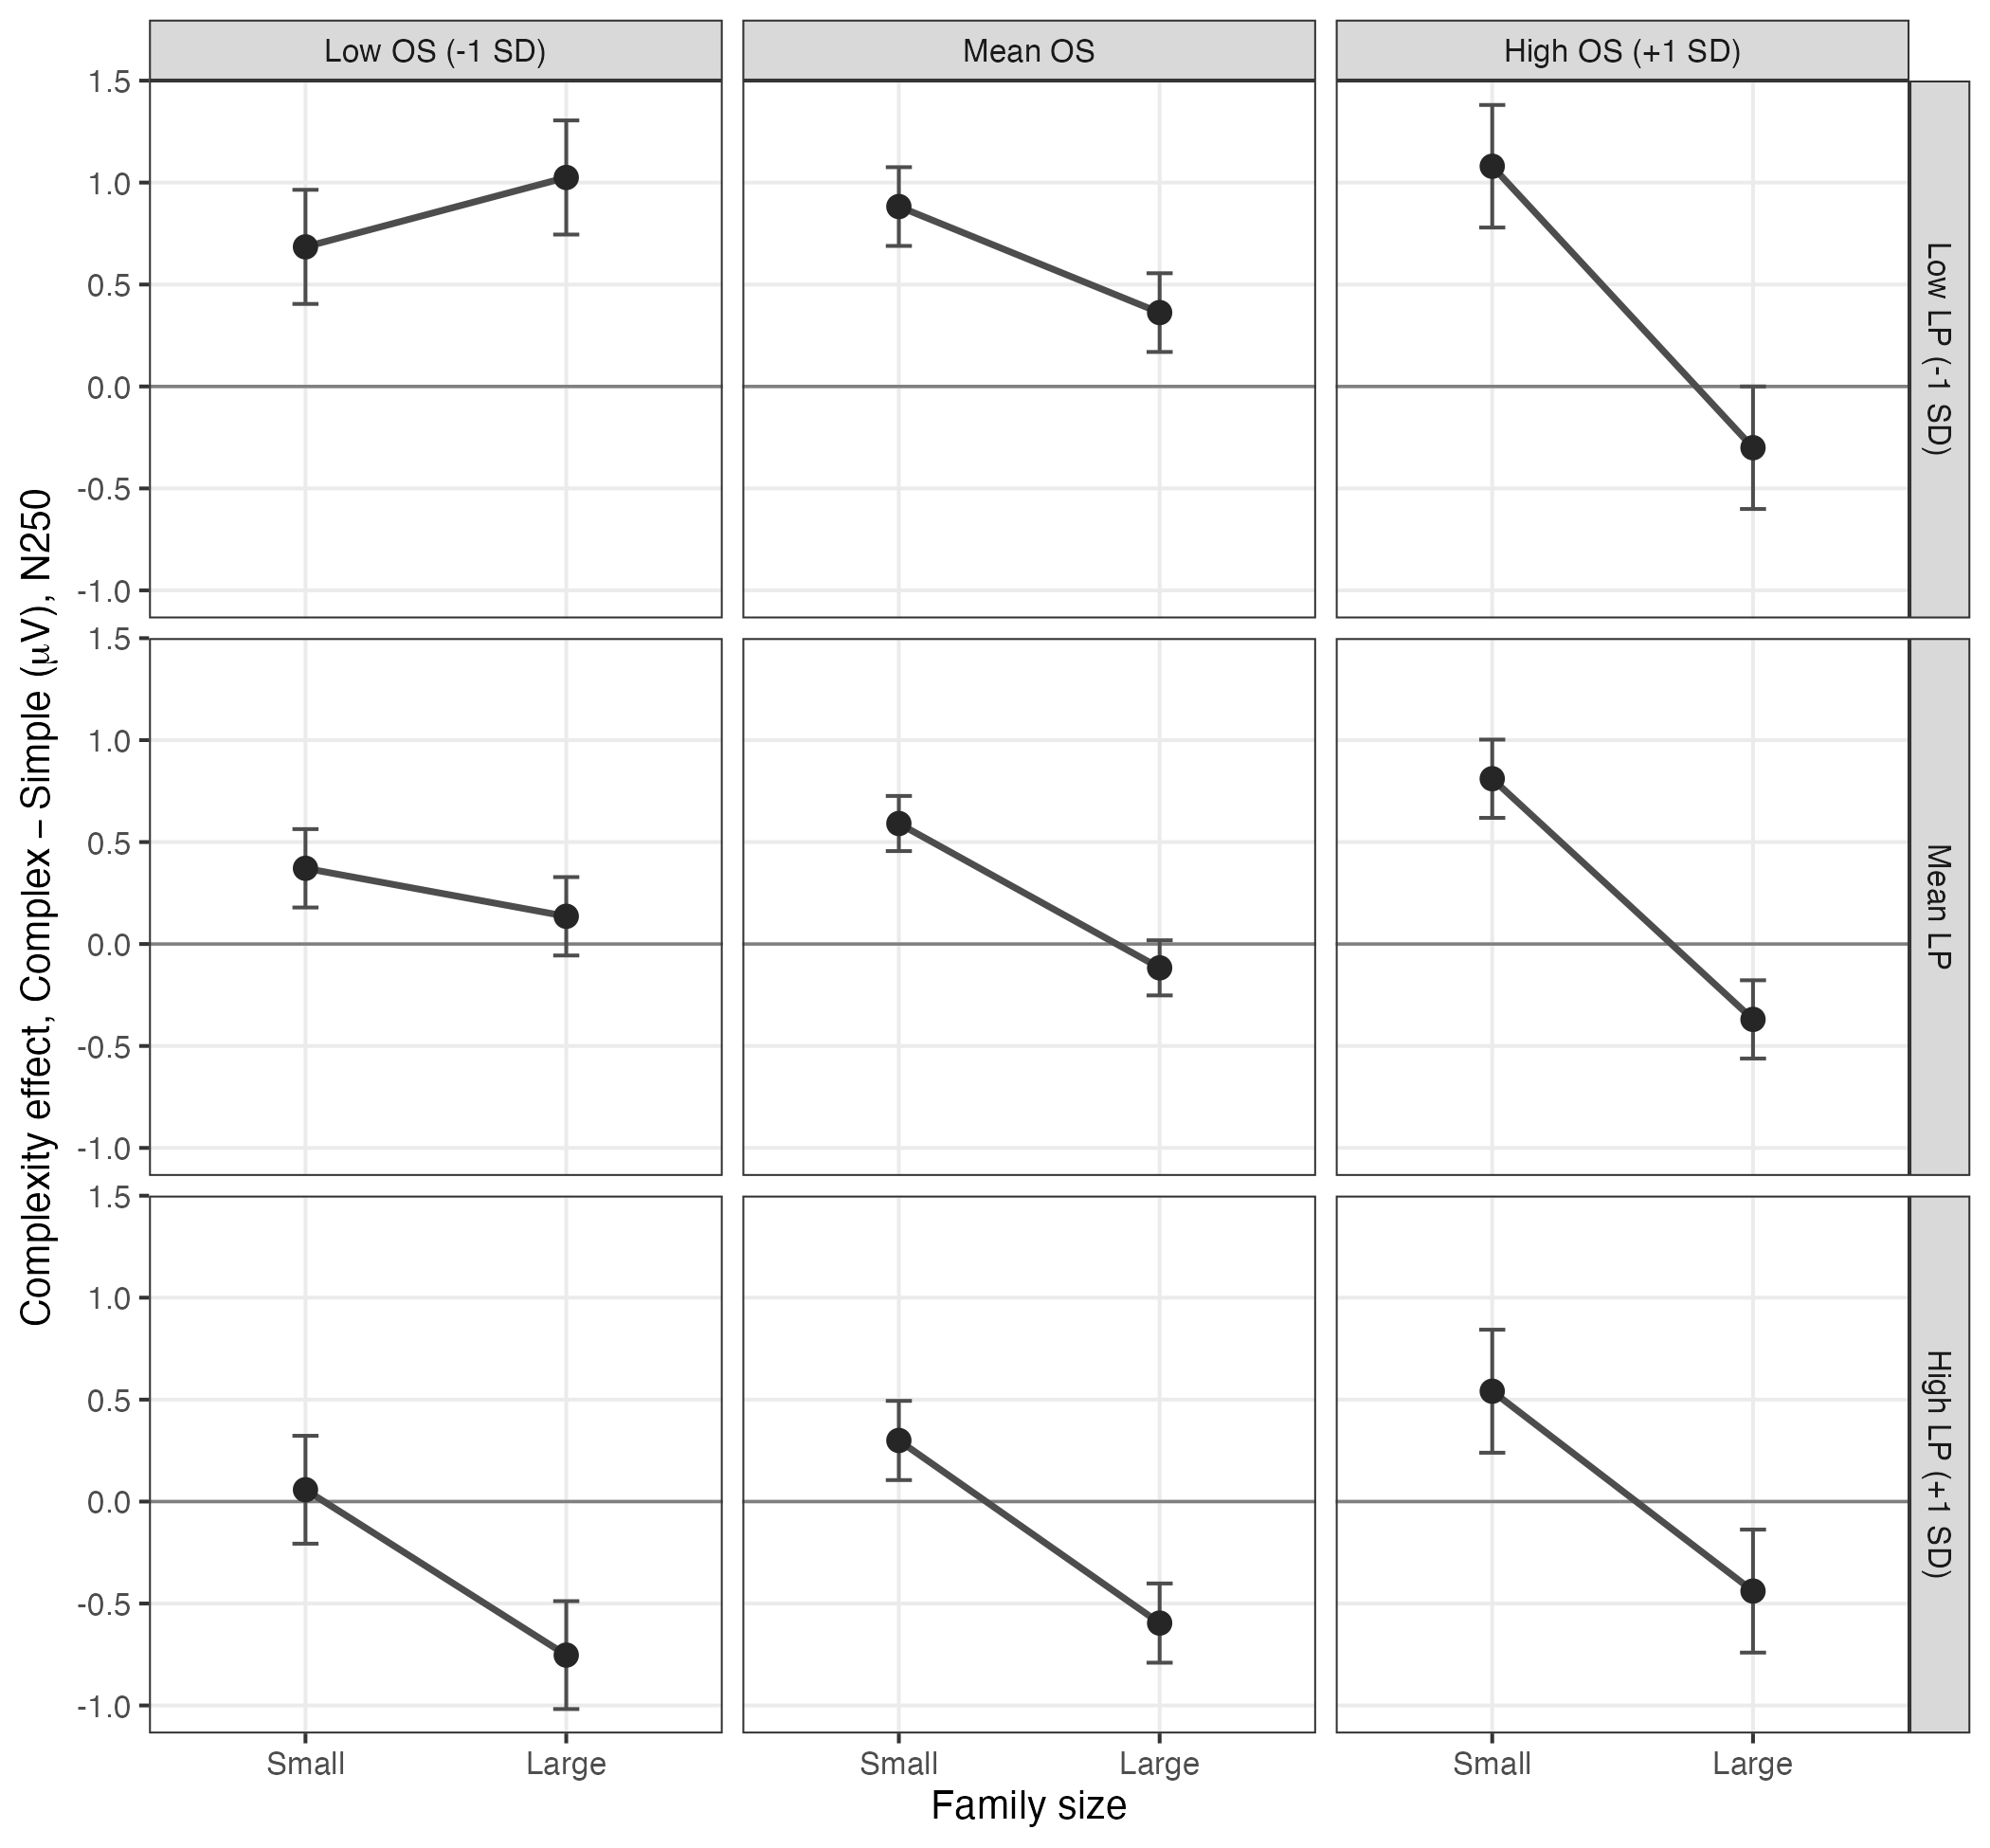
\includegraphics[width=0.85\textwidth]{N250_4way_cxeffect}
	\caption{Complexity effect (Complex $-$ Simple) on nonword N250 amplitude for small- and large-family nonwords, at low ($-1$ SD), mean, and high ($+1$ SD) Language Proficiency (rows) and Orthographic Sensitivity (columns). Estimates and 95\% confidence intervals from the N250 model. A sloping line indicates a Complexity $\times$ Family Size interaction in that cell; positive values indicate less negative amplitudes for complex nonwords.}
	\label{fig:n250}
\end{figure}

\subsection{N400}

Complex nonwords elicited less negative N400 amplitudes than simple nonwords (EMM: Complex $= -0.15\,\mu$V, 95\% CI $[-0.83, 0.53]$; Simple $= -0.54\,\mu$V $[-1.21, 0.14]$), $\beta = 0.389$, $SE = 0.053$, $t(4848) = 7.31$, $p < .001$, $\eta^2_p = .01$, and large-family nonwords elicited more negative amplitudes than small-family nonwords, $\beta = -0.253$, $SE = 0.053$, $t(4848) = -4.75$, $p < .001$, $\eta^2_p = .005$. Neither Language Proficiency, $\beta = -0.088$, $SE = 0.269$, $t(56) = -0.33$, $p = .746$, nor Orthographic Sensitivity, $\beta = 0.519$, $SE = 0.366$, $t(56) = 1.42$, $p = .162$, had a reliable main effect. Unlike at the N250, Complexity did not interact with Family Size for readers at the mean of both dimensions, $\beta = 0.080$, $SE = 0.106$, $t(4848) = 0.75$, $p = .453$.

\paragraph*{Complexity and the individual difference dimensions.} Complexity interacted with both Language Proficiency, $\beta = -0.146$, $SE = 0.042$, $t(4848) = -3.45$, $p < .001$, $\eta^2_p = .002$, and Orthographic Sensitivity, $\beta = 0.160$, $SE = 0.058$, $t(4848) = 2.76$, $p = .006$, $\eta^2_p = .002$, but in opposite directions: averaged over family size, the complexity effect became smaller as Language Proficiency increased and larger as Orthographic Sensitivity increased. With Language Proficiency at its mean, the complexity effect was $0.24\,\mu$V ($SE = 0.08$, $t(4848) = 3.15$, $p = .002$), $0.39\,\mu$V ($SE = 0.05$, $t(4848) = 7.29$, $p < .001$), and $0.54\,\mu$V ($SE = 0.08$, $t(4848) = 7.12$, $p < .001$) at low, mean, and high Orthographic Sensitivity. Family Size also interacted with Language Proficiency, $\beta = 0.247$, $SE = 0.042$, $t(4848) = 5.82$, $p < .001$, $\eta^2_p = .007$. The Complexity $\times$ Language Proficiency and Family Size $\times$ Language Proficiency terms were qualified by the three-way interaction below.

\paragraph*{Language Proficiency and the Complexity $\times$ Family Size interaction.} There was a Complexity $\times$ Family Size $\times$ Language Proficiency interaction, $\beta = -0.333$, $SE = 0.085$, $t(4848) = -3.92$, $p < .001$, $\eta^2_p = .003$. With Orthographic Sensitivity at its mean, the Complexity $\times$ Family Size contrast was positive at low Language Proficiency ($0.50\,\mu$V, $SE = 0.15$, $t(4848) = 3.28$, $p = .001$), absent at mean Language Proficiency ($0.08\,\mu$V, $SE = 0.11$, $t(4848) = 0.71$, $p = .477$), and negative at high Language Proficiency ($-0.35\,\mu$V, $SE = 0.15$, $t(4848) = -2.27$, $p = .023$). The null Complexity $\times$ Family Size term at the mean thus reflects opposite interactions at the two ends of the Language Proficiency range.

Higher Language Proficiency reduced the complexity effect for large-family nonwords only. For large-family nonwords, the complexity effect was $0.82\,\mu$V ($SE = 0.11$, $t(4848) = 7.67$, $p < .001$), $0.43\,\mu$V ($SE = 0.08$, $t(4848) = 5.66$, $p < .001$), and $0.03\,\mu$V ($SE = 0.11$, $t(4848) = 0.26$, $p = .797$) at low, mean, and high Language Proficiency (slope $= -0.31$, $SE = 0.06$, $t(4848) = -5.16$, $p < .001$). For small-family nonwords it was present at all three levels ($0.33\,\mu$V, $SE = 0.11$, $t(4848) = 3.03$, $p = .003$; $0.35\,\mu$V, $SE = 0.08$, $t(4848) = 4.66$, $p < .001$; $0.38\,\mu$V, $SE = 0.11$, $t(4848) = 3.47$, $p < .001$) and did not change with Language Proficiency (slope $= 0.02$, $SE = 0.06$, $t(4848) = 0.32$, $p = .748$). Unlike at the N250, the complexity effect was reduced to zero but did not reverse. The cell means (Figure~\ref{fig:n400cells}) show that this pattern came mainly from the simple nonwords: at low Language Proficiency, large-family simple nonwords were more negative than small-family simple nonwords, and at high Language Proficiency this order reversed, whereas the difference between large- and small-family complex nonwords was smaller and did not reverse.

The Complexity $\times$ Family Size $\times$ Orthographic Sensitivity interaction was not significant, $\beta = 0.122$, $SE = 0.116$, $t(4848) = 1.05$, $p = .292$.

\paragraph*{Four-way interaction.} The Language Proficiency three-way interaction was qualified by a four-way interaction, $\beta = 0.269$, $SE = 0.107$, $t(4848) = 2.51$, $p = .012$, $\eta^2_p = .001$; a likelihood-ratio test confirmed that the four-way term improved fit, $\chi^2(1) = 6.31$, $p = .012$. Table~\ref{tab:n400nw} gives the Complexity $\times$ Family Size interaction contrast across the two dimensions, and Figure~\ref{fig:n400} shows the corresponding complexity effects. The contrast was positive for readers low in Language Proficiency who were low or average in Orthographic Sensitivity ($0.70\,\mu$V, $t(4848) = 3.18$, $p = .002$; $0.50\,\mu$V, $t(4848) = 3.28$, $p = .001$), and negative for readers high in Language Proficiency who were low or average in Orthographic Sensitivity ($-0.79\,\mu$V, $t(4848) = -3.77$, $p < .001$; $-0.35\,\mu$V, $t(4848) = -2.27$, $p = .023$). It was not significant in the remaining five cells, including all three cells for readers high in Orthographic Sensitivity (all $p \geq .20$). Language Proficiency therefore changed the interaction only when Orthographic Sensitivity was low or average: the Language Proficiency slope of the interaction contrast was $-0.58$ at low Orthographic Sensitivity ($SE = 0.12$, $t(4848) = -4.89$, $p < .001$), $-0.33$ at mean Orthographic Sensitivity ($SE = 0.09$, $t(4848) = -3.87$, $p < .001$), and $-0.08$ at high Orthographic Sensitivity ($SE = 0.14$, $t(4848) = -0.56$, $p = .575$). Correspondingly, the Orthographic Sensitivity slope was $-0.22$ at low Language Proficiency ($SE = 0.18$, $t(4848) = -1.19$, $p = .235$), $0.13$ at mean Language Proficiency ($SE = 0.12$, $t(4848) = 1.10$, $p = .274$), and $0.47$ at high Language Proficiency ($SE = 0.18$, $t(4848) = 2.69$, $p = .007$). No other interaction was significant (all $p \geq .15$).

\begin{table}[htbp]
	\centering
	\small
	\caption{Complexity $\times$ Family Size interaction contrast for nonword N400 amplitude across Language Proficiency and Orthographic Sensitivity. Each cell gives the complexity effect (Complex $-$ Simple) for large-family nonwords minus the complexity effect for small-family nonwords, in $\mu$V, with its $t$ value in parentheses ($df = 4848$). Positive values indicate a larger complexity effect for large-family nonwords; negative values indicate a smaller one. Levels as in Table~\ref{tab:n250nw}.}
	\label{tab:n400nw}
	\begin{tabular}{lccc}
		\toprule
		& OS $-1$ SD & OS mean & OS $+1$ SD \\
		\midrule
		LP $-1$ SD & $0.70$ ($3.18$) & $0.50$ ($3.28$) & $0.30$ ($1.25$) \\
		LP mean & $-0.04$ ($-0.28$) & $0.08$ ($0.71$) & $0.19$ ($1.28$) \\
		LP $+1$ SD & $-0.79$ ($-3.77$) & $-0.35$ ($-2.27$) & $0.09$ ($0.38$) \\
		\bottomrule
	\end{tabular}
\end{table}

\begin{figure}[htbp]
	\centering
	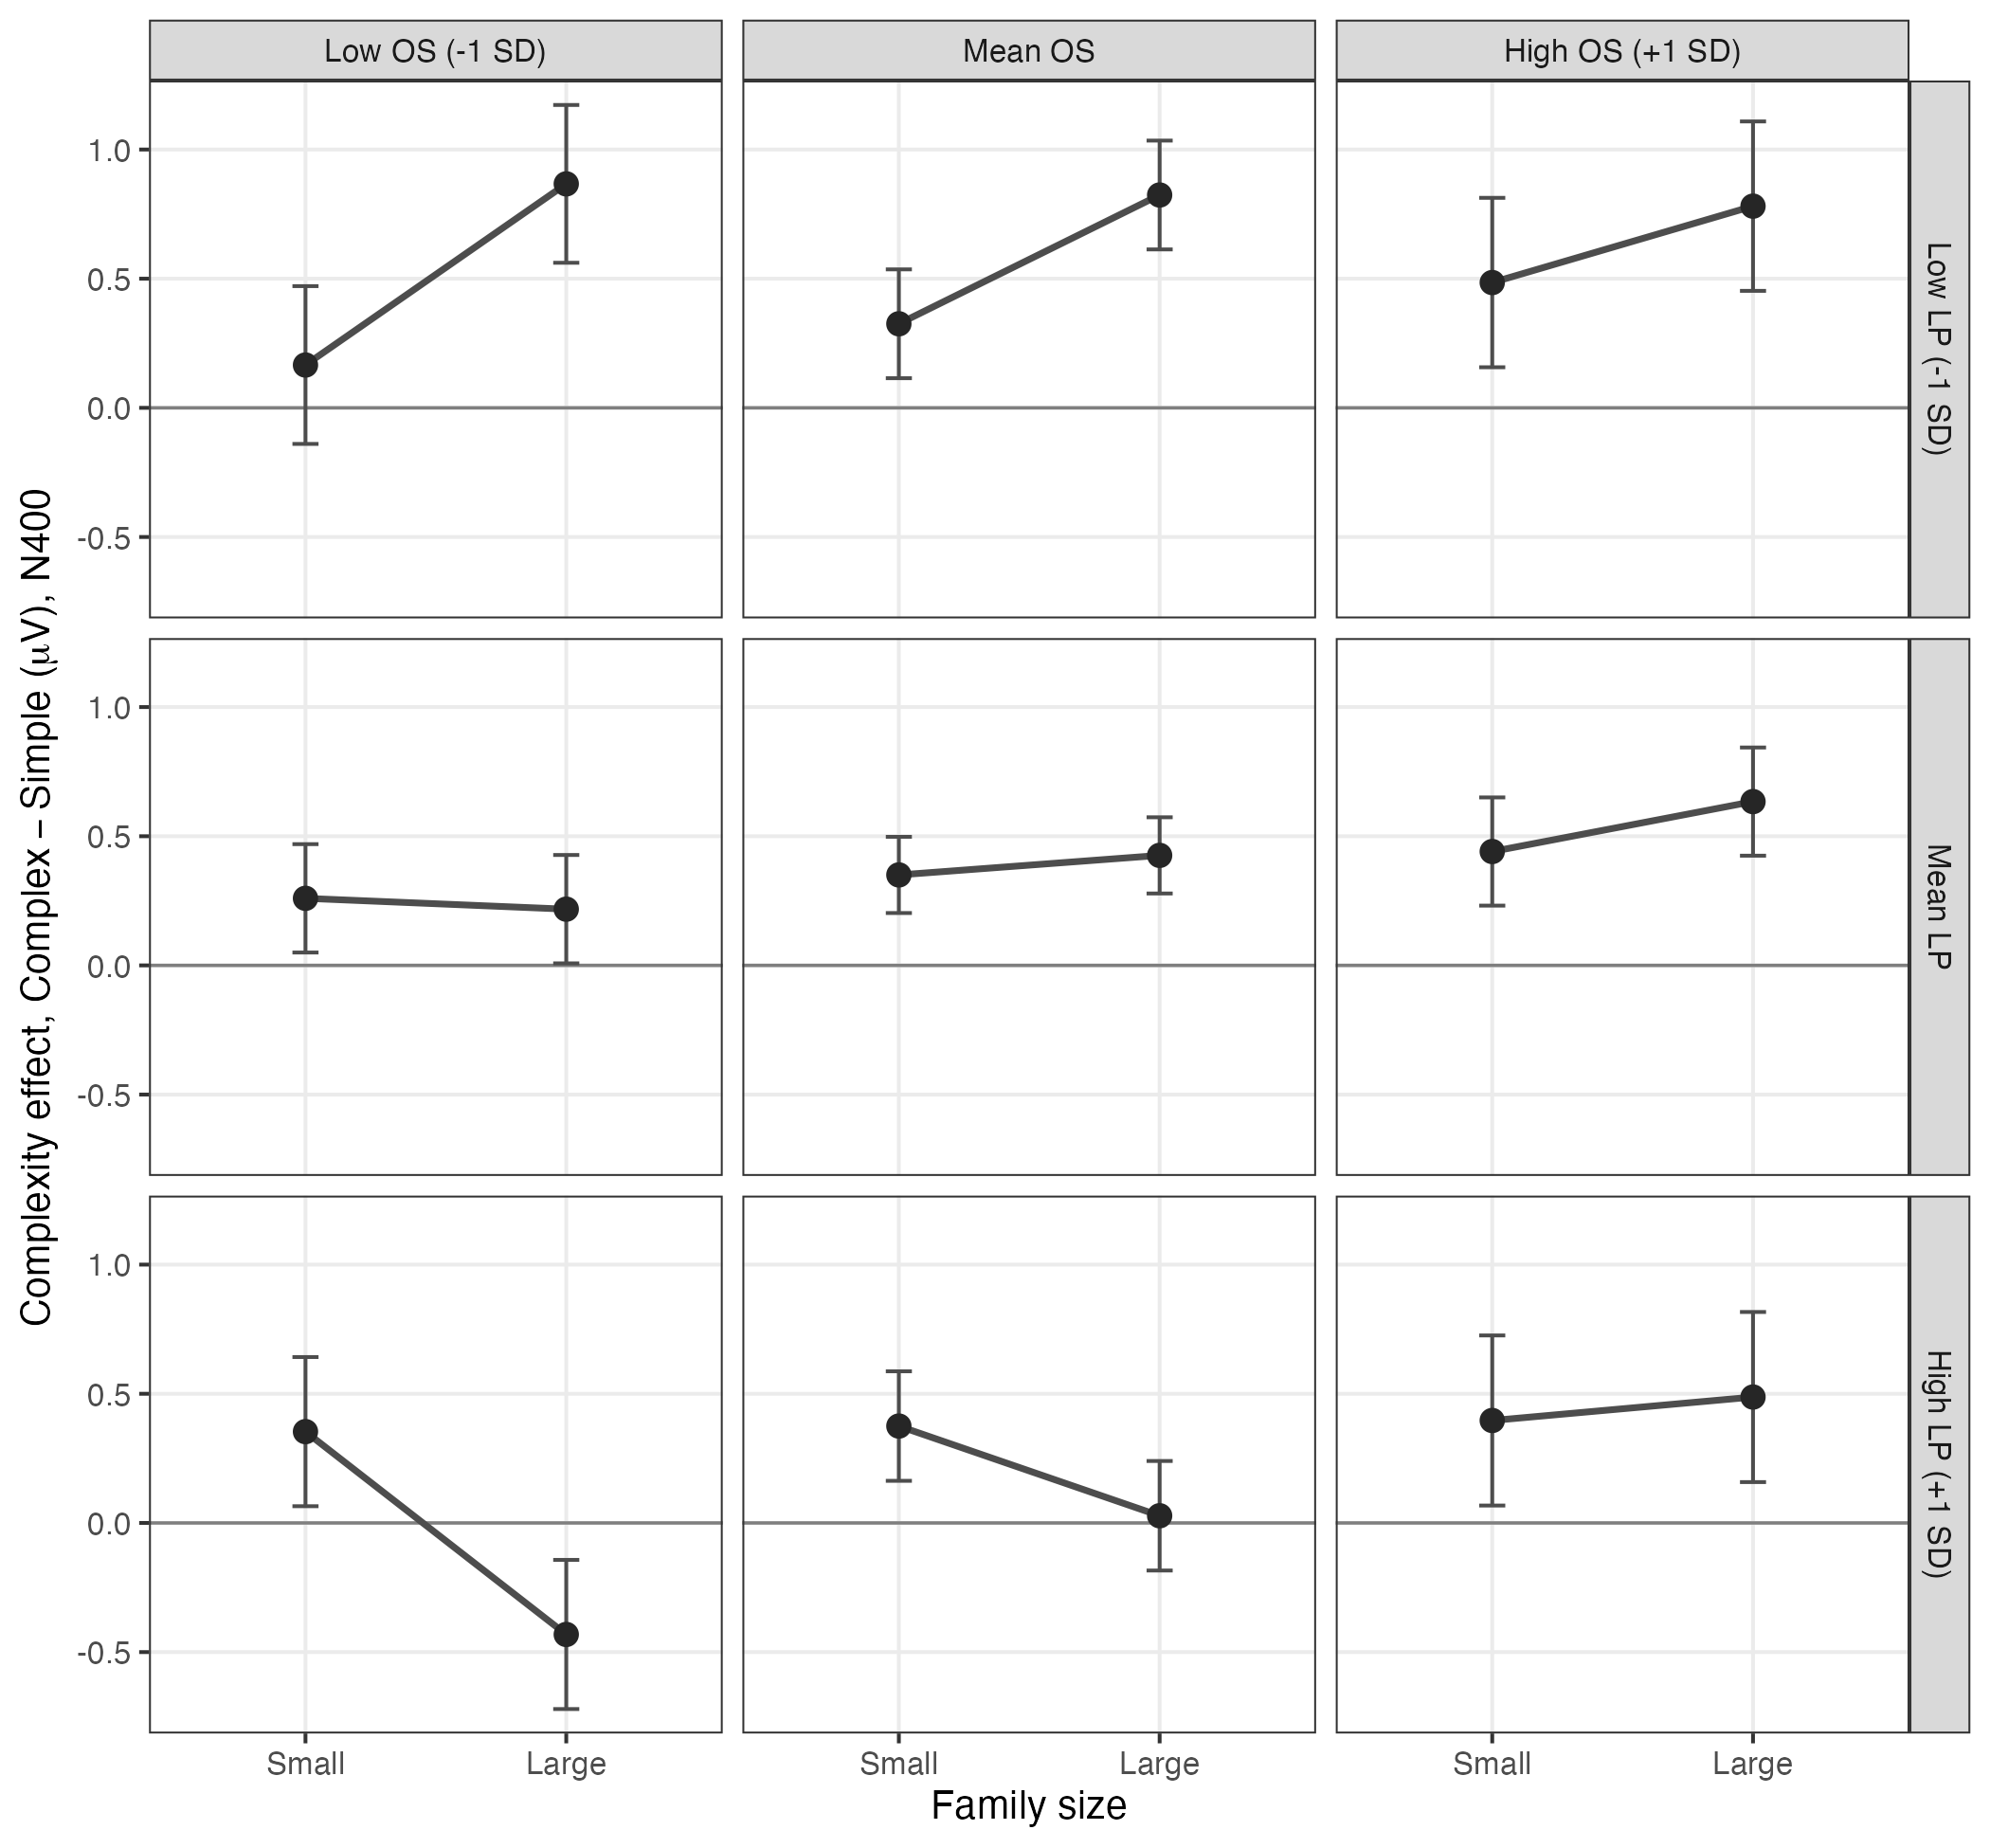
\includegraphics[width=0.85\textwidth]{N400_4way_cxeffect}
	\caption{Complexity effect (Complex $-$ Simple) on nonword N400 amplitude for small- and large-family nonwords, at low ($-1$ SD), mean, and high ($+1$ SD) Language Proficiency (rows) and Orthographic Sensitivity (columns). Estimates and 95\% confidence intervals from the N400 model.}
	\label{fig:n400}
\end{figure}

\begin{figure}[htbp]
	\centering
	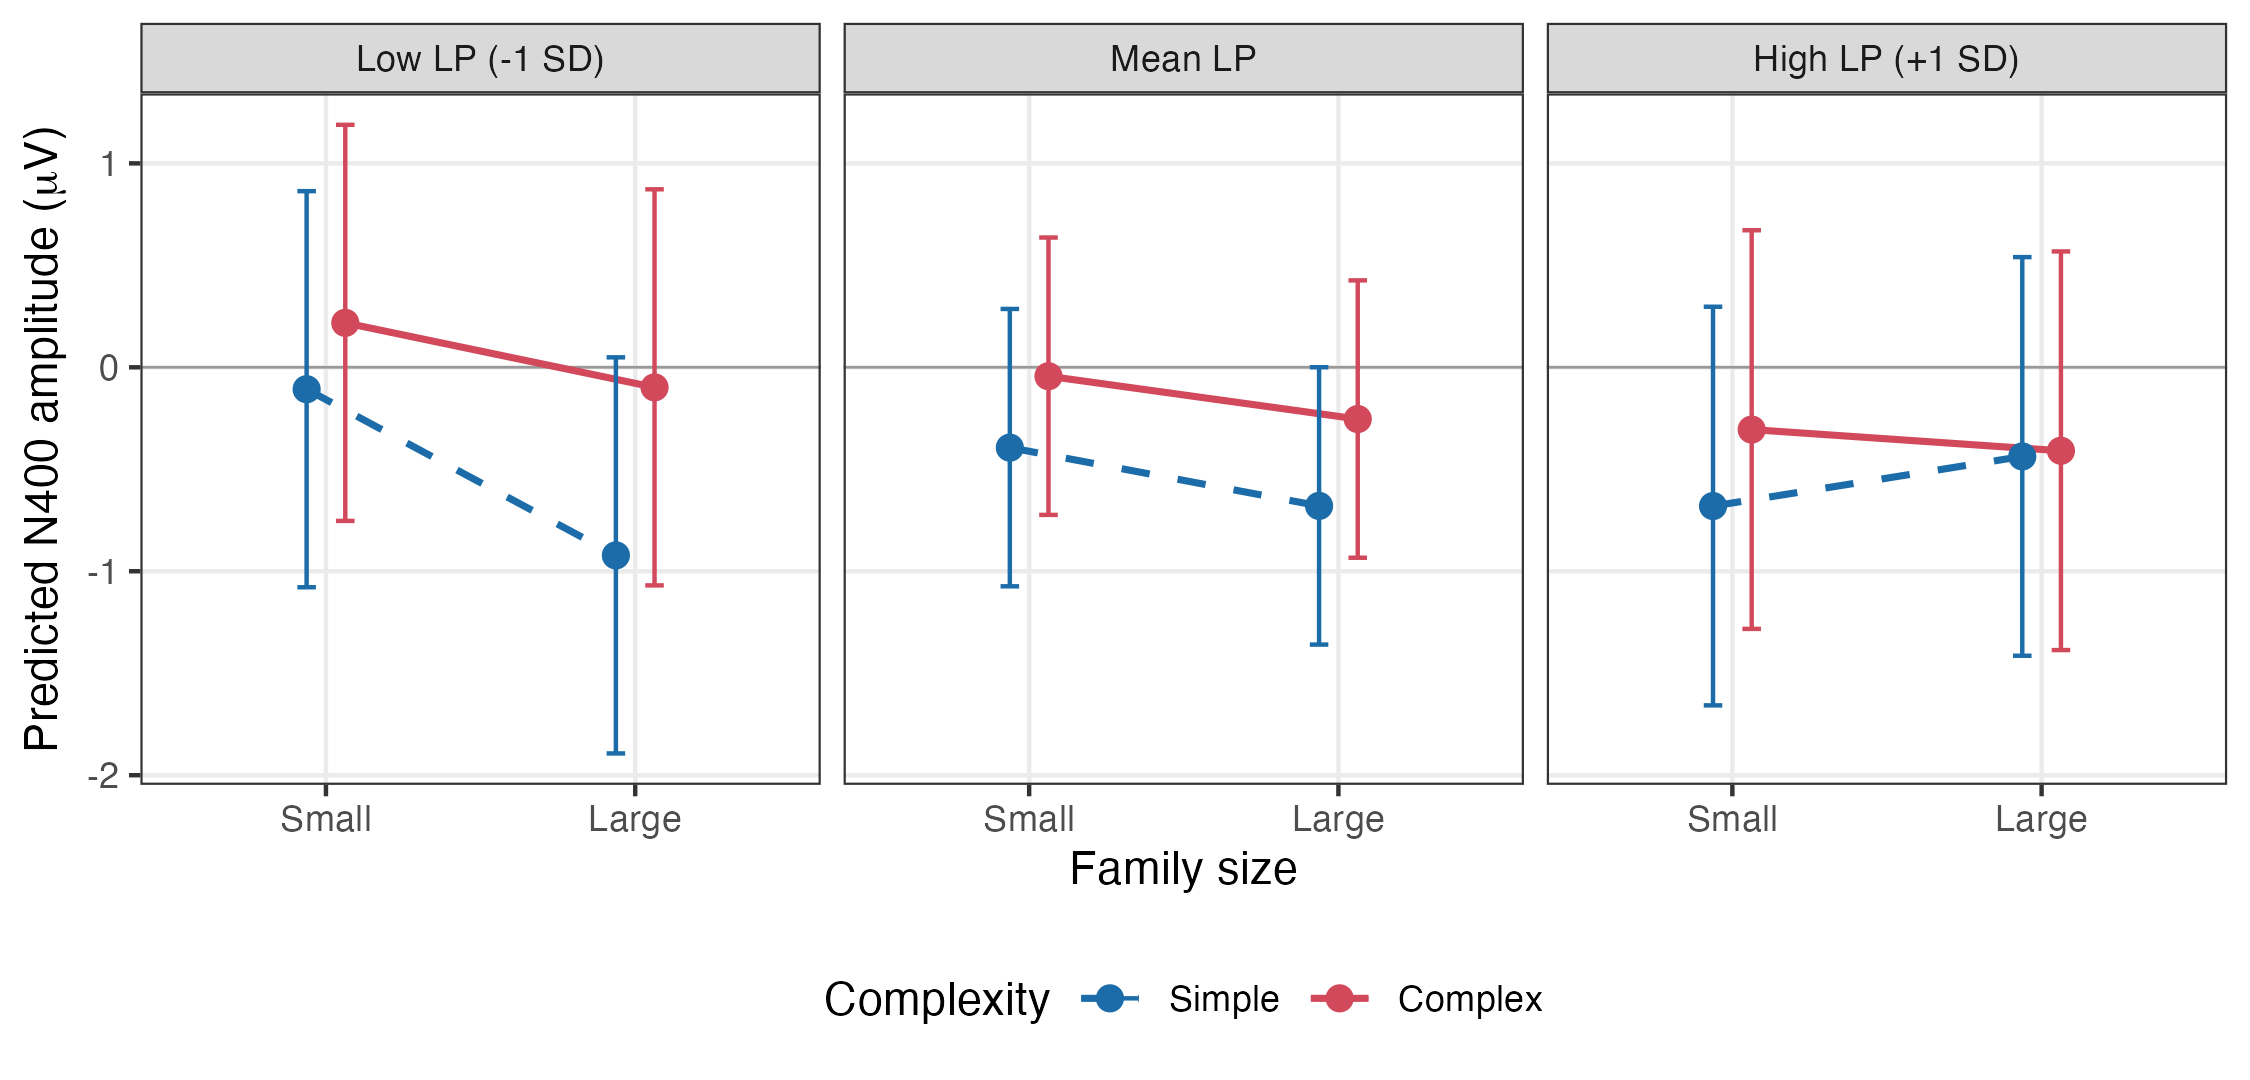
\includegraphics[width=0.9\textwidth]{Figure_N400_CxFSxLP_cells}
	\caption{Predicted nonword N400 amplitude by Family Size and Complexity at low ($-1$ SD), mean, and high ($+1$ SD) Language Proficiency, with Orthographic Sensitivity at its mean. Estimated marginal means and 95\% confidence intervals from the N400 model.}
	\label{fig:n400cells}
\end{figure}

\subsection{Differences Between the N250 and the N400}

In the combined model, removing every term that contained both Orthographic Sensitivity and Time Window reduced fit, $\chi^2(8) = 24.42$, $p = .002$, as did removing every term that contained both Language Proficiency and Time Window, $\chi^2(8) = 28.00$, $p < .001$. The contributions of both dimensions therefore differed between the two components. The individual terms (Table~\ref{tab:fixed}, right-hand columns) show that they differed in different ways. The model also confirmed that the Complexity $\times$ Family Size interaction differed between components, $\beta = 0.780$, $SE = 0.144$, $t(9696) = 5.40$, $p < .001$: it was present at the N250 and absent at the N400 for readers at the mean of both dimensions.

\paragraph*{Orthographic Sensitivity.} The highest-order term containing both Orthographic Sensitivity and Time Window that reached significance was Complexity $\times$ Family Size $\times$ Orthographic Sensitivity $\times$ Time Window, $\beta = 0.637$, $SE = 0.157$, $t(9696) = 4.05$, $p < .001$; the Complexity $\times$ Orthographic Sensitivity $\times$ Time Window term, $\beta = 0.181$, $SE = 0.079$, $t(9696) = 2.30$, $p = .021$, is contained within it. The change between components was confined to large-family nonwords (Figure~\ref{fig:window}A). For these nonwords, with Language Proficiency at its mean, the slope of the complexity effect on Orthographic Sensitivity was negative at the N250 ($-0.27$, $SE = 0.08$, $t(9696) = -3.47$, $p < .001$) and positive at the N400 ($0.22$, $SE = 0.08$, $t(9696) = 2.86$, $p = .004$), a difference of $0.50$ ($SE = 0.11$, $t(9696) = 4.48$, $p < .001$). For small-family nonwords, the slope was $0.24$ at the N250 ($SE = 0.08$, $t(9696) = 3.02$, $p = .003$) and $0.10$ at the N400 ($SE = 0.08$, $t(9696) = 1.24$, $p = .214$), and did not differ reliably between components ($-0.14$, $SE = 0.11$, $t(9696) = -1.25$, $p = .210$). The direction of Orthographic Sensitivity's influence on the complexity effect for large-family nonwords therefore reversed between the N250 and the N400.

\paragraph*{Language Proficiency.} No term containing Language Proficiency and Time Window was significant above the three-way level (Complexity $\times$ Family Size $\times$ Language Proficiency $\times$ Time Window, $\beta = -0.183$, $SE = 0.115$, $t(9696) = -1.59$, $p = .113$). Two three-way terms were significant. First, Complexity $\times$ Language Proficiency $\times$ Time Window, $\beta = 0.156$, $SE = 0.058$, $t(9696) = 2.71$, $p = .007$: averaged over family size, the slope of the complexity effect on Language Proficiency was $-0.30$ at the N250 ($SE = 0.04$, $t(9696) = -7.36$, $p < .001$) and $-0.15$ at the N400 ($SE = 0.04$, $t(9696) = -3.57$, $p < .001$), a difference of $0.16$ ($SE = 0.06$, $t(9696) = 2.68$, $p = .007$; Figure~\ref{fig:window}B). Second, Family Size $\times$ Language Proficiency $\times$ Time Window, $\beta = 0.208$, $SE = 0.058$, $t(9696) = 3.62$, $p < .001$: averaged over complexity, the slope of the family size effect on Language Proficiency was $0.04$ at the N250 ($SE = 0.04$, $t(9696) = 0.98$, $p = .330$) and $0.25$ at the N400 ($SE = 0.04$, $t(9696) = 6.07$, $p < .001$), a difference of $0.21$ ($SE = 0.06$, $t(9696) = 3.60$, $p < .001$; Figure~\ref{fig:window}C). Higher Language Proficiency reduced the complexity effect at both components, but less at the N400, and it changed the family size effect at the N400 but not at the N250.

The Complexity $\times$ Family Size $\times$ Language Proficiency $\times$ Orthographic Sensitivity interaction, averaged over the two components, was significant, $\beta = 0.298$, $SE = 0.073$, $t(9696) = 4.09$, $p < .001$, and did not differ between them, $\beta = -0.057$, $SE = 0.146$, $t(9696) = -0.39$, $p = .697$, consistent with its significance in both component models.

\begin{figure}[htbp]
	\centering
	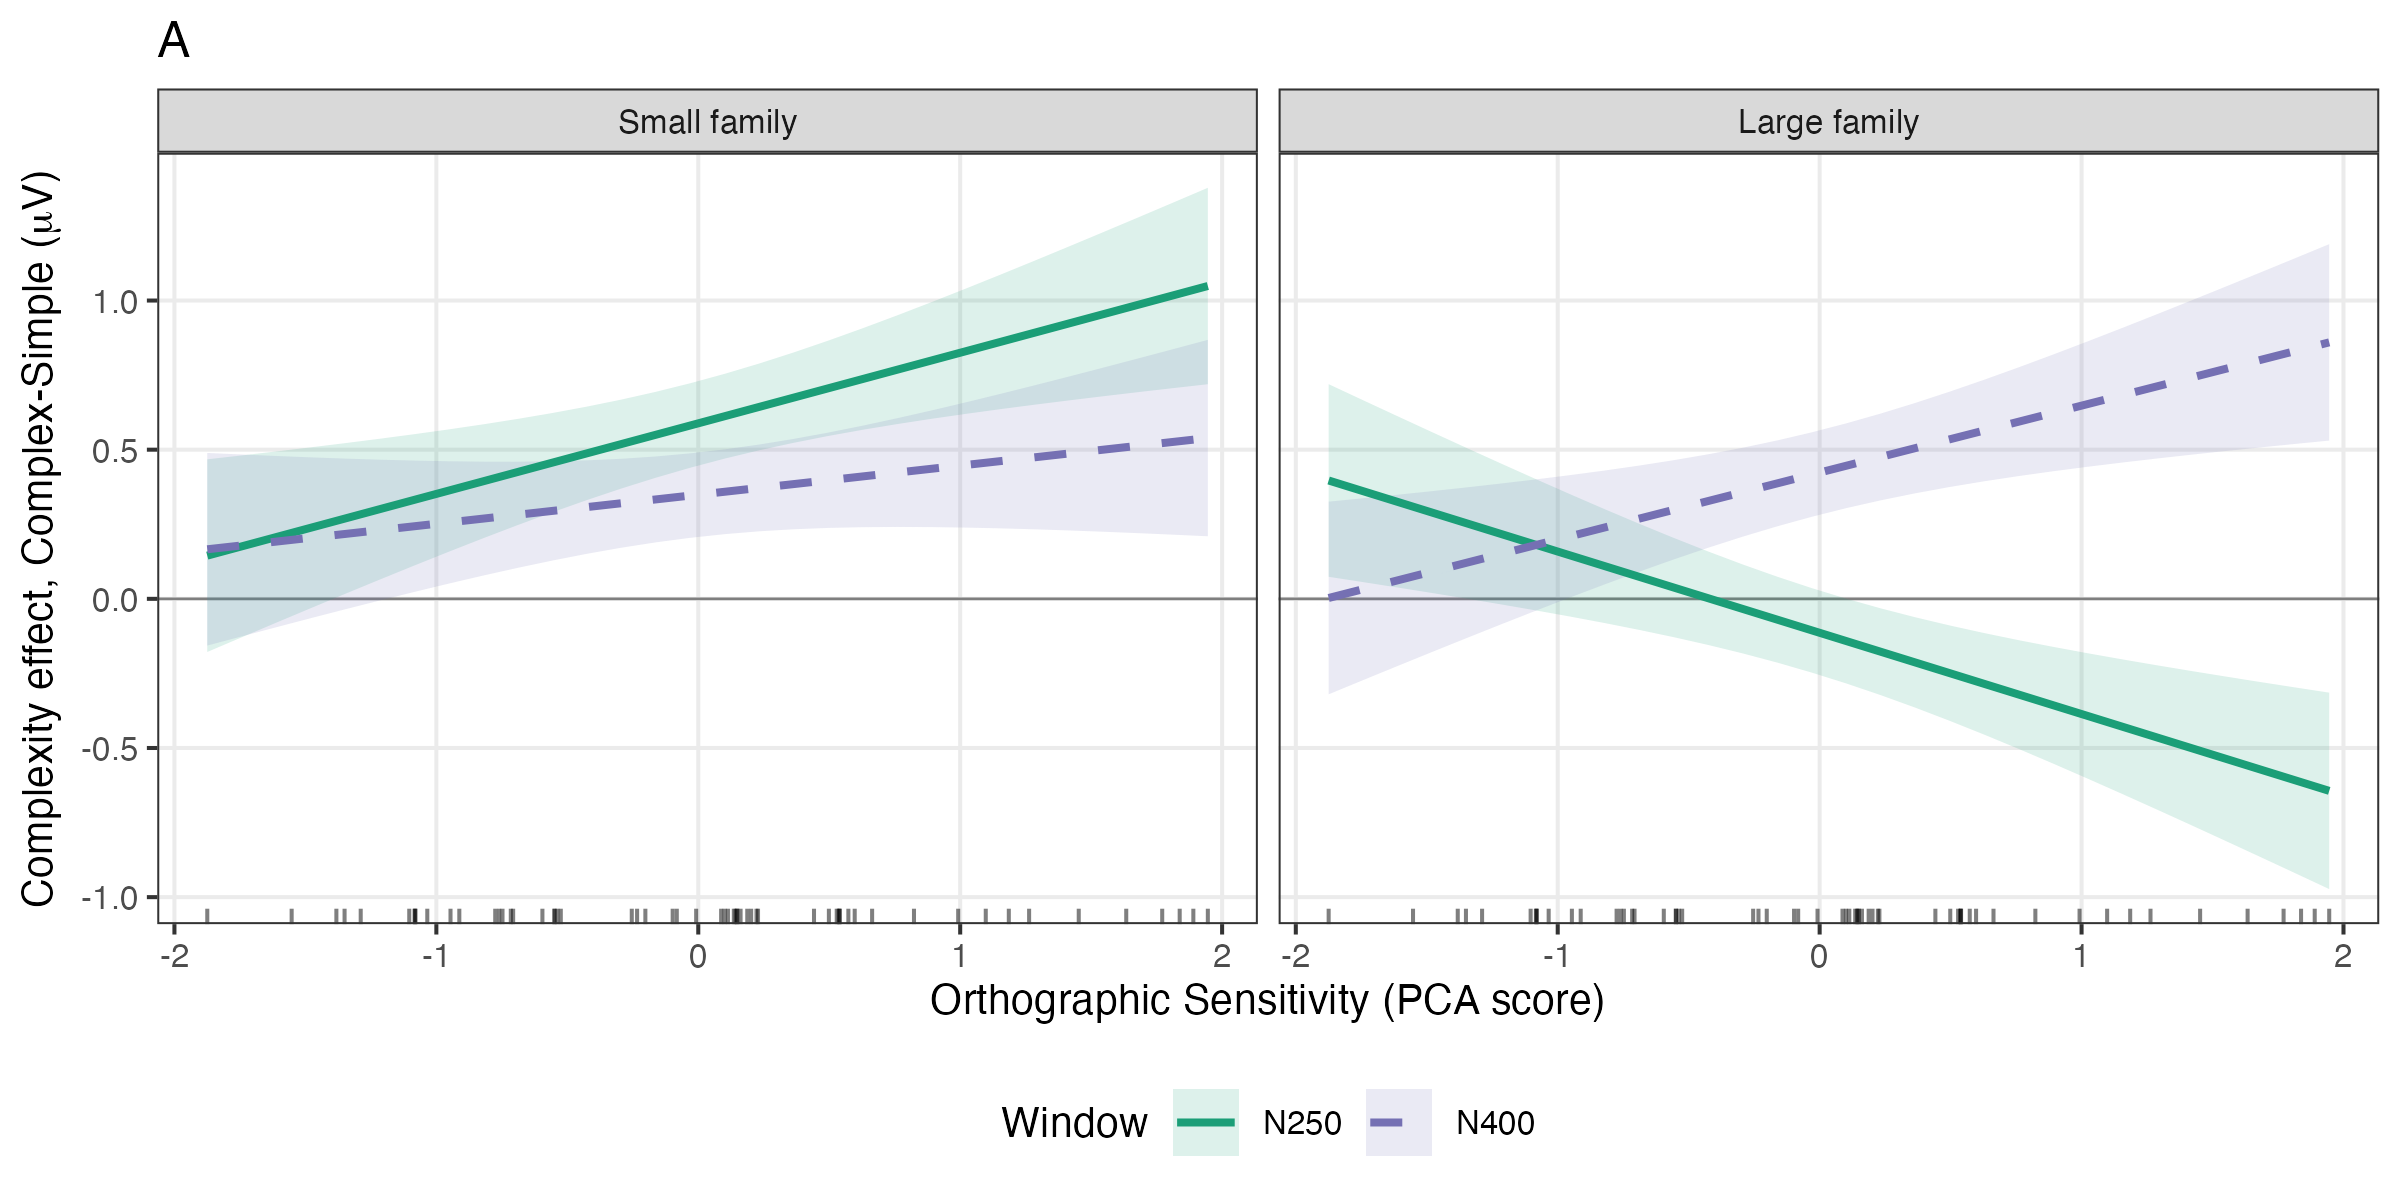
\includegraphics[width=0.95\textwidth]{Window_A_CxFSxOS}\\[1ex]
	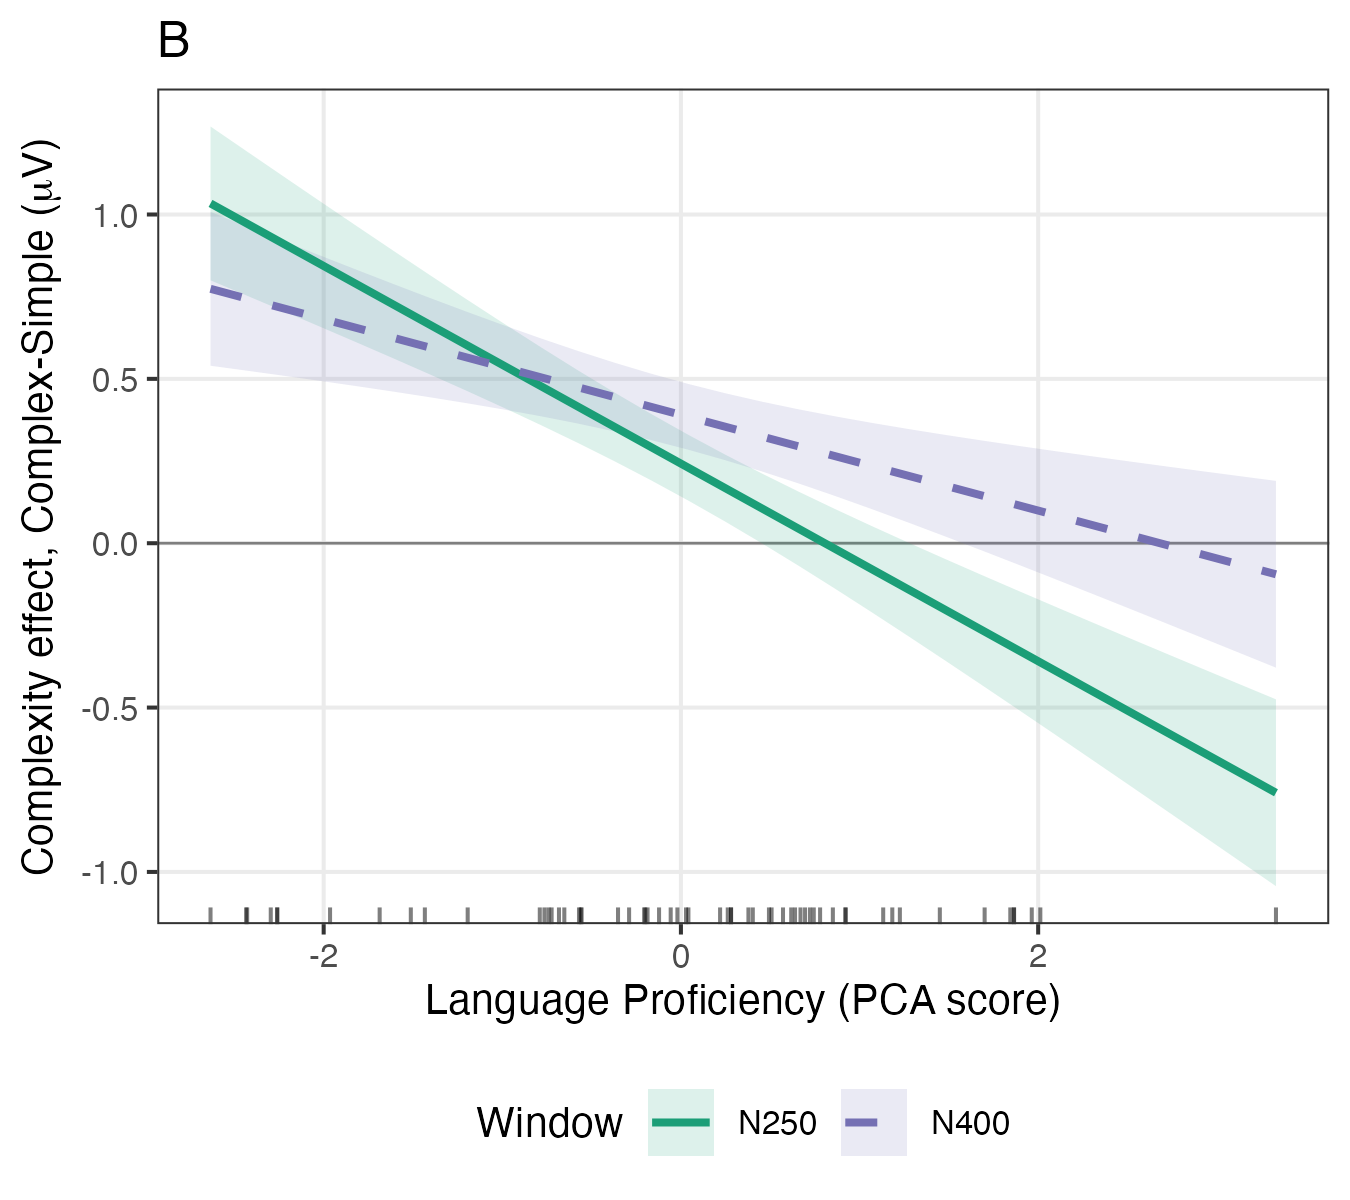
\includegraphics[width=0.48\textwidth]{Window_B_CxLP}\hfill
	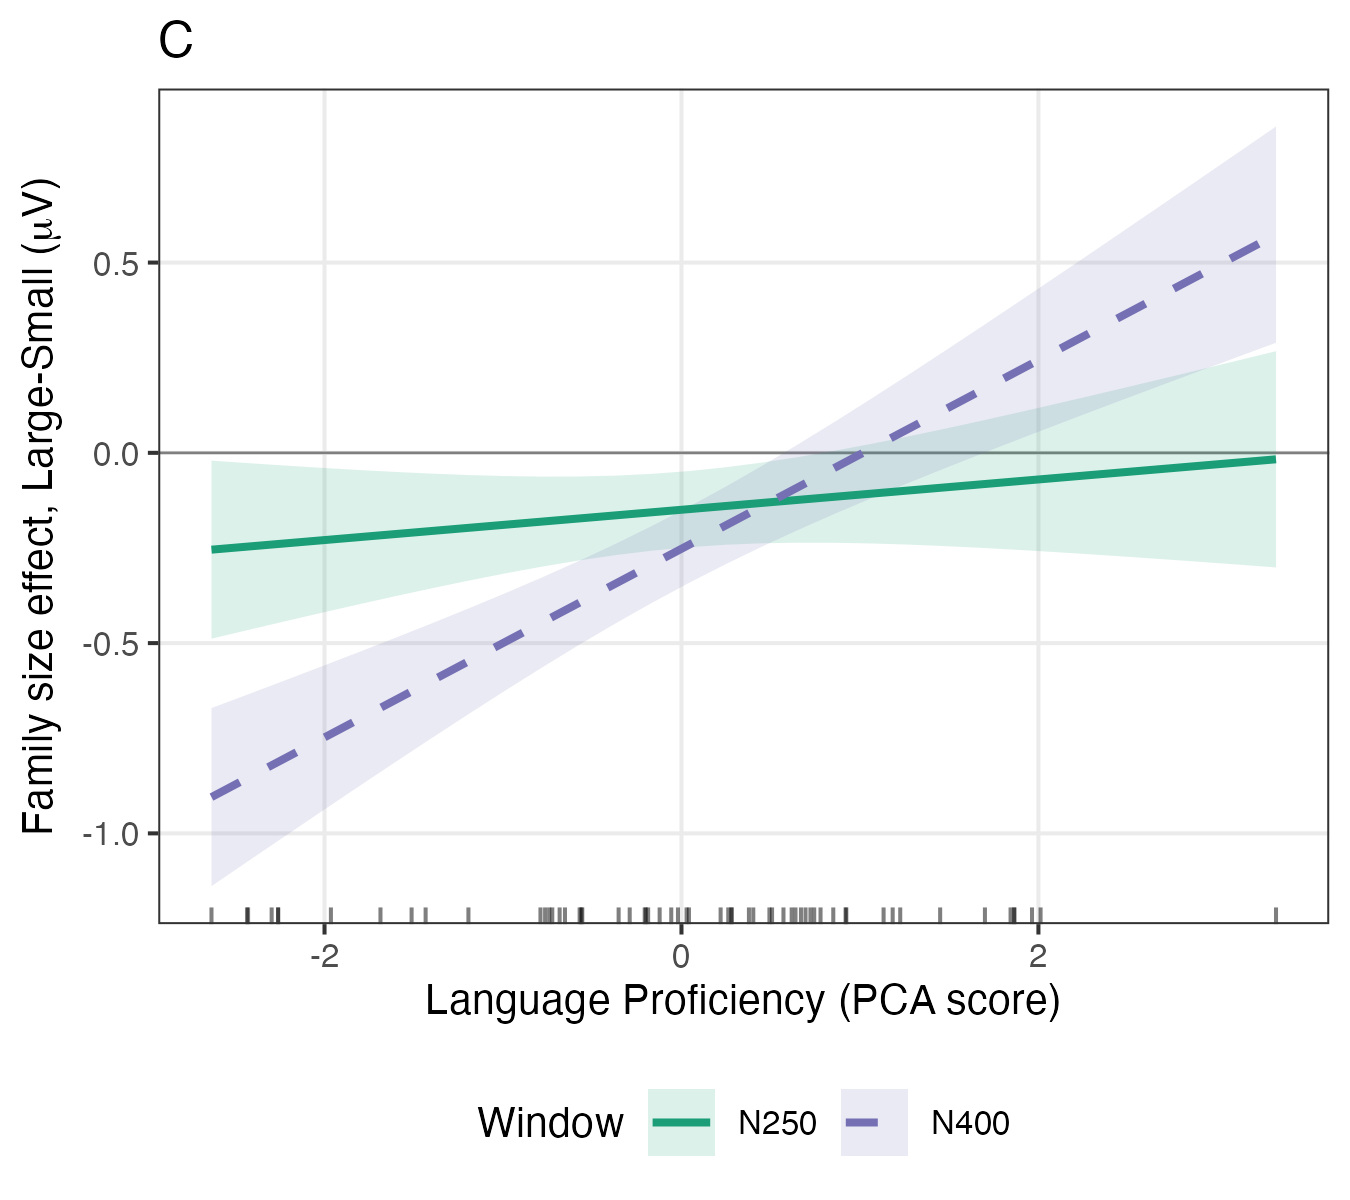
\includegraphics[width=0.48\textwidth]{Window_C_FSxLP}
	\caption{Effects that differed between the N250 and the N400 in the combined model, plotted across the observed range of each dimension. (A) Complexity effect (Complex $-$ Simple) as a function of Orthographic Sensitivity for small- and large-family nonwords, with Language Proficiency at its mean. (B) Complexity effect as a function of Language Proficiency, averaged over family size, with Orthographic Sensitivity at its mean. (C) Family size effect (Large $-$ Small) as a function of Language Proficiency, averaged over complexity, with Orthographic Sensitivity at its mean. Lines with different slopes indicate an effect that changes between components. Shaded bands are 95\% confidence intervals; tick marks show individual participants' scores.}
	\label{fig:window}
\end{figure}

\subsection{Summary}

At the N250, complex nonwords elicited less negative amplitudes than simple nonwords when the base had a small family; for readers at the mean of both dimensions, this complexity effect was absent for large-family nonwords. Orthographic Sensitivity enlarged this Complexity $\times$ Family Size interaction, so that readers high in Orthographic Sensitivity showed a reversed complexity effect for large-family nonwords. Language Proficiency enlarged the interaction only for readers low in Orthographic Sensitivity, and Orthographic Sensitivity had no further effect for readers high in Language Proficiency. At the N400, the Complexity $\times$ Family Size interaction was absent at average skill levels but ran in opposite directions at the two ends of the Language Proficiency range: high Language Proficiency eliminated, without reversing, the complexity effect for large-family nonwords. This modulation by Language Proficiency was present for readers low or average in Orthographic Sensitivity and absent for readers high in it. The combined model showed that the contributions of both dimensions differed between components, in different ways: the influence of Orthographic Sensitivity on the complexity effect for large-family nonwords reversed direction from the N250 to the N400, whereas the influence of Language Proficiency on the complexity effect weakened from the N250 to the N400 and its influence on the family size effect emerged only at the N400.
	
	\section{Discussion}
	
	
	\section*{Conflict of Interest Statement}
	The authors declare that the research was conducted in the absence of any commercial or financial relationships that could be construed as a potential conflict of interest.
	
	\section*{Author Contributions}
	JM: Conceptualization, Methodology, Software, Validation, Formal analysis, Resources, Data curation, Visualization, Writing – original draft, Writing – review \& editing, Supervision.
	EK: Methodology, Software, Investigation, Data curation, Writing – original draft, Writing – review \& editing, Supervision.
	FG: Methodology, Software, Investigation, Data curation.
	JP: Investigation, Data curation, Writing – review \& editing
	TR: Investigation, Data curation, Writing – review \& editing
	EM: Investigation, Data curation, Writing – review \& editing
	CR-M: Investigation, Data curation, Writing – review \& editing
	NA: Investigation, Data curation, Writing – review \& editing
	
	All authors contributed to the article and approved the submitted version.
	
	\section*{Funding}
	Research reported in this manuscript was supported by the Rhode Island IDeA Network of Biomedical Research Excellence, funded by the National Institute of General Medical Sciences of the National Institutes of Health under grant number P20GM103430. Additional support for student researchers (Joemari Pulido, Tess Rooney, Natalia Alzate, Ethan Moore, and Crismar Ramos-Marte) and for data collection was provided through the Center for Engaged Learning at Providence College and a series of Hampshire College Faculty Development Grants awarded to Dr. Morris during her tenure at that institution. The funders had no role in study design, data collection and analysis, decision to publish, or preparation of the manuscript.
	
	
	\section*{Acknowledgments}
	We thank Sophie Fulghum, Dylan Palumbo, Maeve Garrity, Aleksandra Kurylowicz, Sarah Debian, Aleksandra Saneff, Kenny Diaz, and Kiley Vallee for their assistance with participant recruitment and data collection.
	
	\section*{Supplemental Data}
	\href{http://home.frontiersin.org/about/author-guidelines#SupplementaryMaterial}{Supplementary Material} should be uploaded separately on submission, if there are Supplementary Figures, please include the caption in the same file as the figure. LaTeX Supplementary Material templates can be found in the Frontiers LaTeX folder.
	
	\section*{Data Availability Statement}
	The datasets [GENERATED/ANALYZED] for this study can be found in the [NAME OF REPOSITORY] [LINK].
	% Please see the availability of data guidelines for more information, at https://www.frontiersin.org/about/author-guidelines#AvailabilityofData
	
	\bibliographystyle{Frontiers-Harvard} % Many Frontiers journals use the Harvard referencing system (Author-date), to find the style and resources for the journal you are submitting to—https://zendesk.frontiersin.org/hc/en-us/articles/360017860337-Frontiers-Reference-Styles-by-Journal. For Humanities and Social Sciences articles please include page numbers in the in-text citations 
	%\bibliographystyle{Frontiers-Vancouver} % Many Frontiers journals use the numbered referencing system, to find the style and resources for the journal you are submitting to—https://zendesk.frontiersin.org/hc/en-us/articles/360017860337-Frontiers-Reference-Styles-by-Journal
	\bibliography{M21_LDT.bib}
	
	
	\end{document}